% !TeX root = ..\..\rapport_13_1.tex
\section{Programdesign}
\subsection{Klassediagram af programdesign}
Programmets klasser inddeles i lag som ses på \cref{fig:classLayers}.
\begin{figure}
    \centering
    \caption{TaskFusion klasser inddelt i lag}\label{fig:classLayers}
    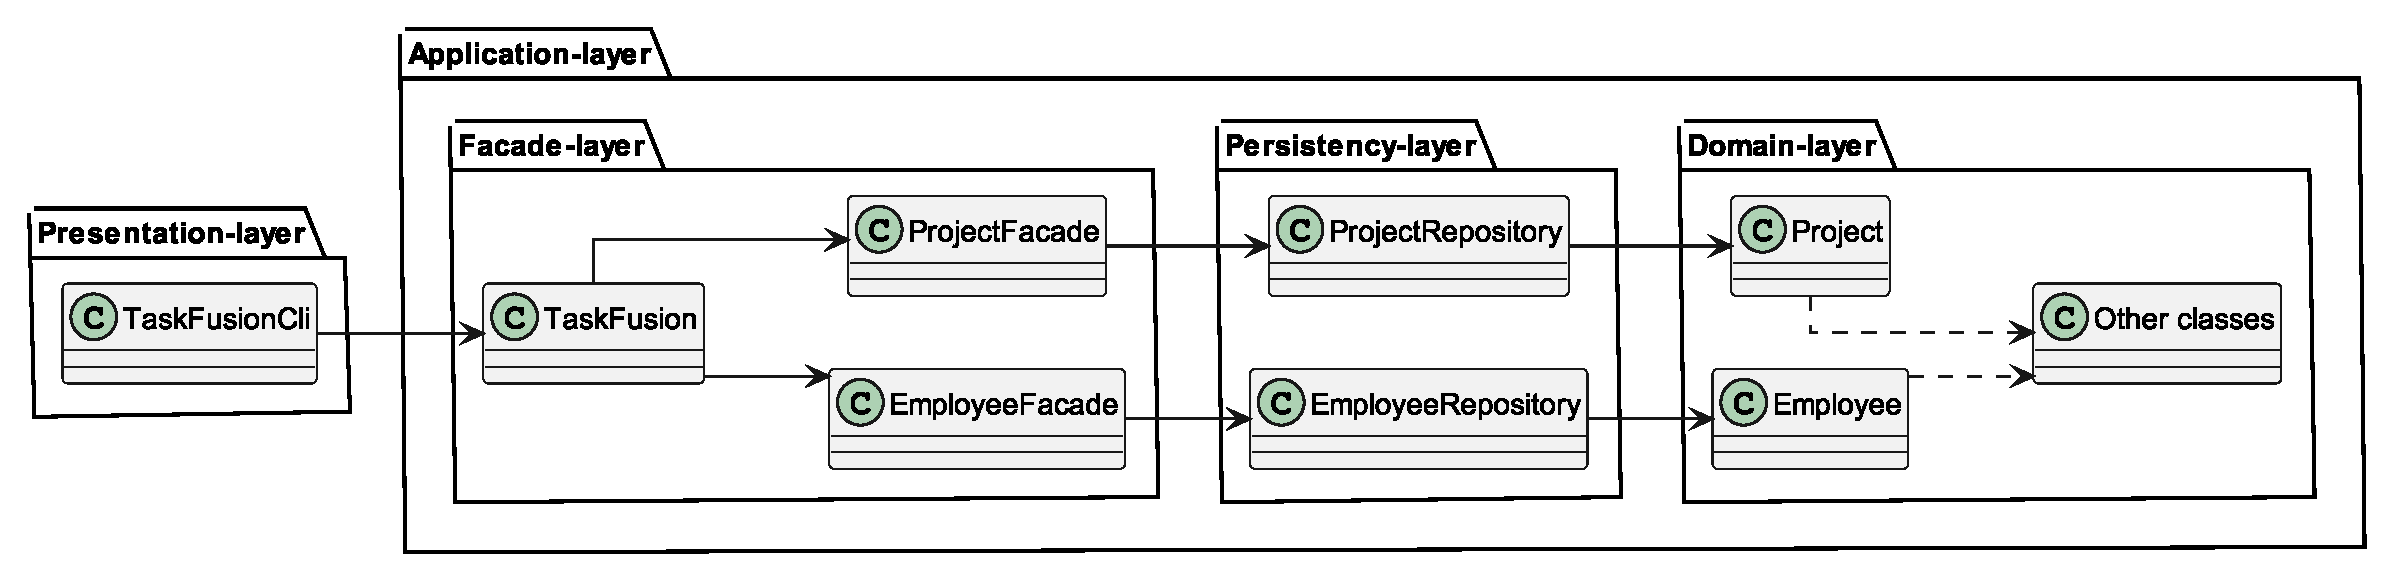
\includegraphics[width=\textwidth]{TaskFusion/out/assets/diagrams/class_persistency_layer/ClassDiagram_layer.eps}
\end{figure}
TaskFusionCLI opretter et TaskFusion objekt som opretter ProjectFacade og EmployeeFacade. Her kan TaskFusion sende metodekald til to singletons:
\begin{itemize}
    \item ProjectRepository
    \item EmployeeRepository
\end{itemize}
Metodekaldene opretter og ændrer felter i domain laget, som ses på \cref{fig:domainLayer}.
\begin{figure}
    \centering
    \caption{TaskFusion klasser i domain laget}\label{fig:domainLayer}
    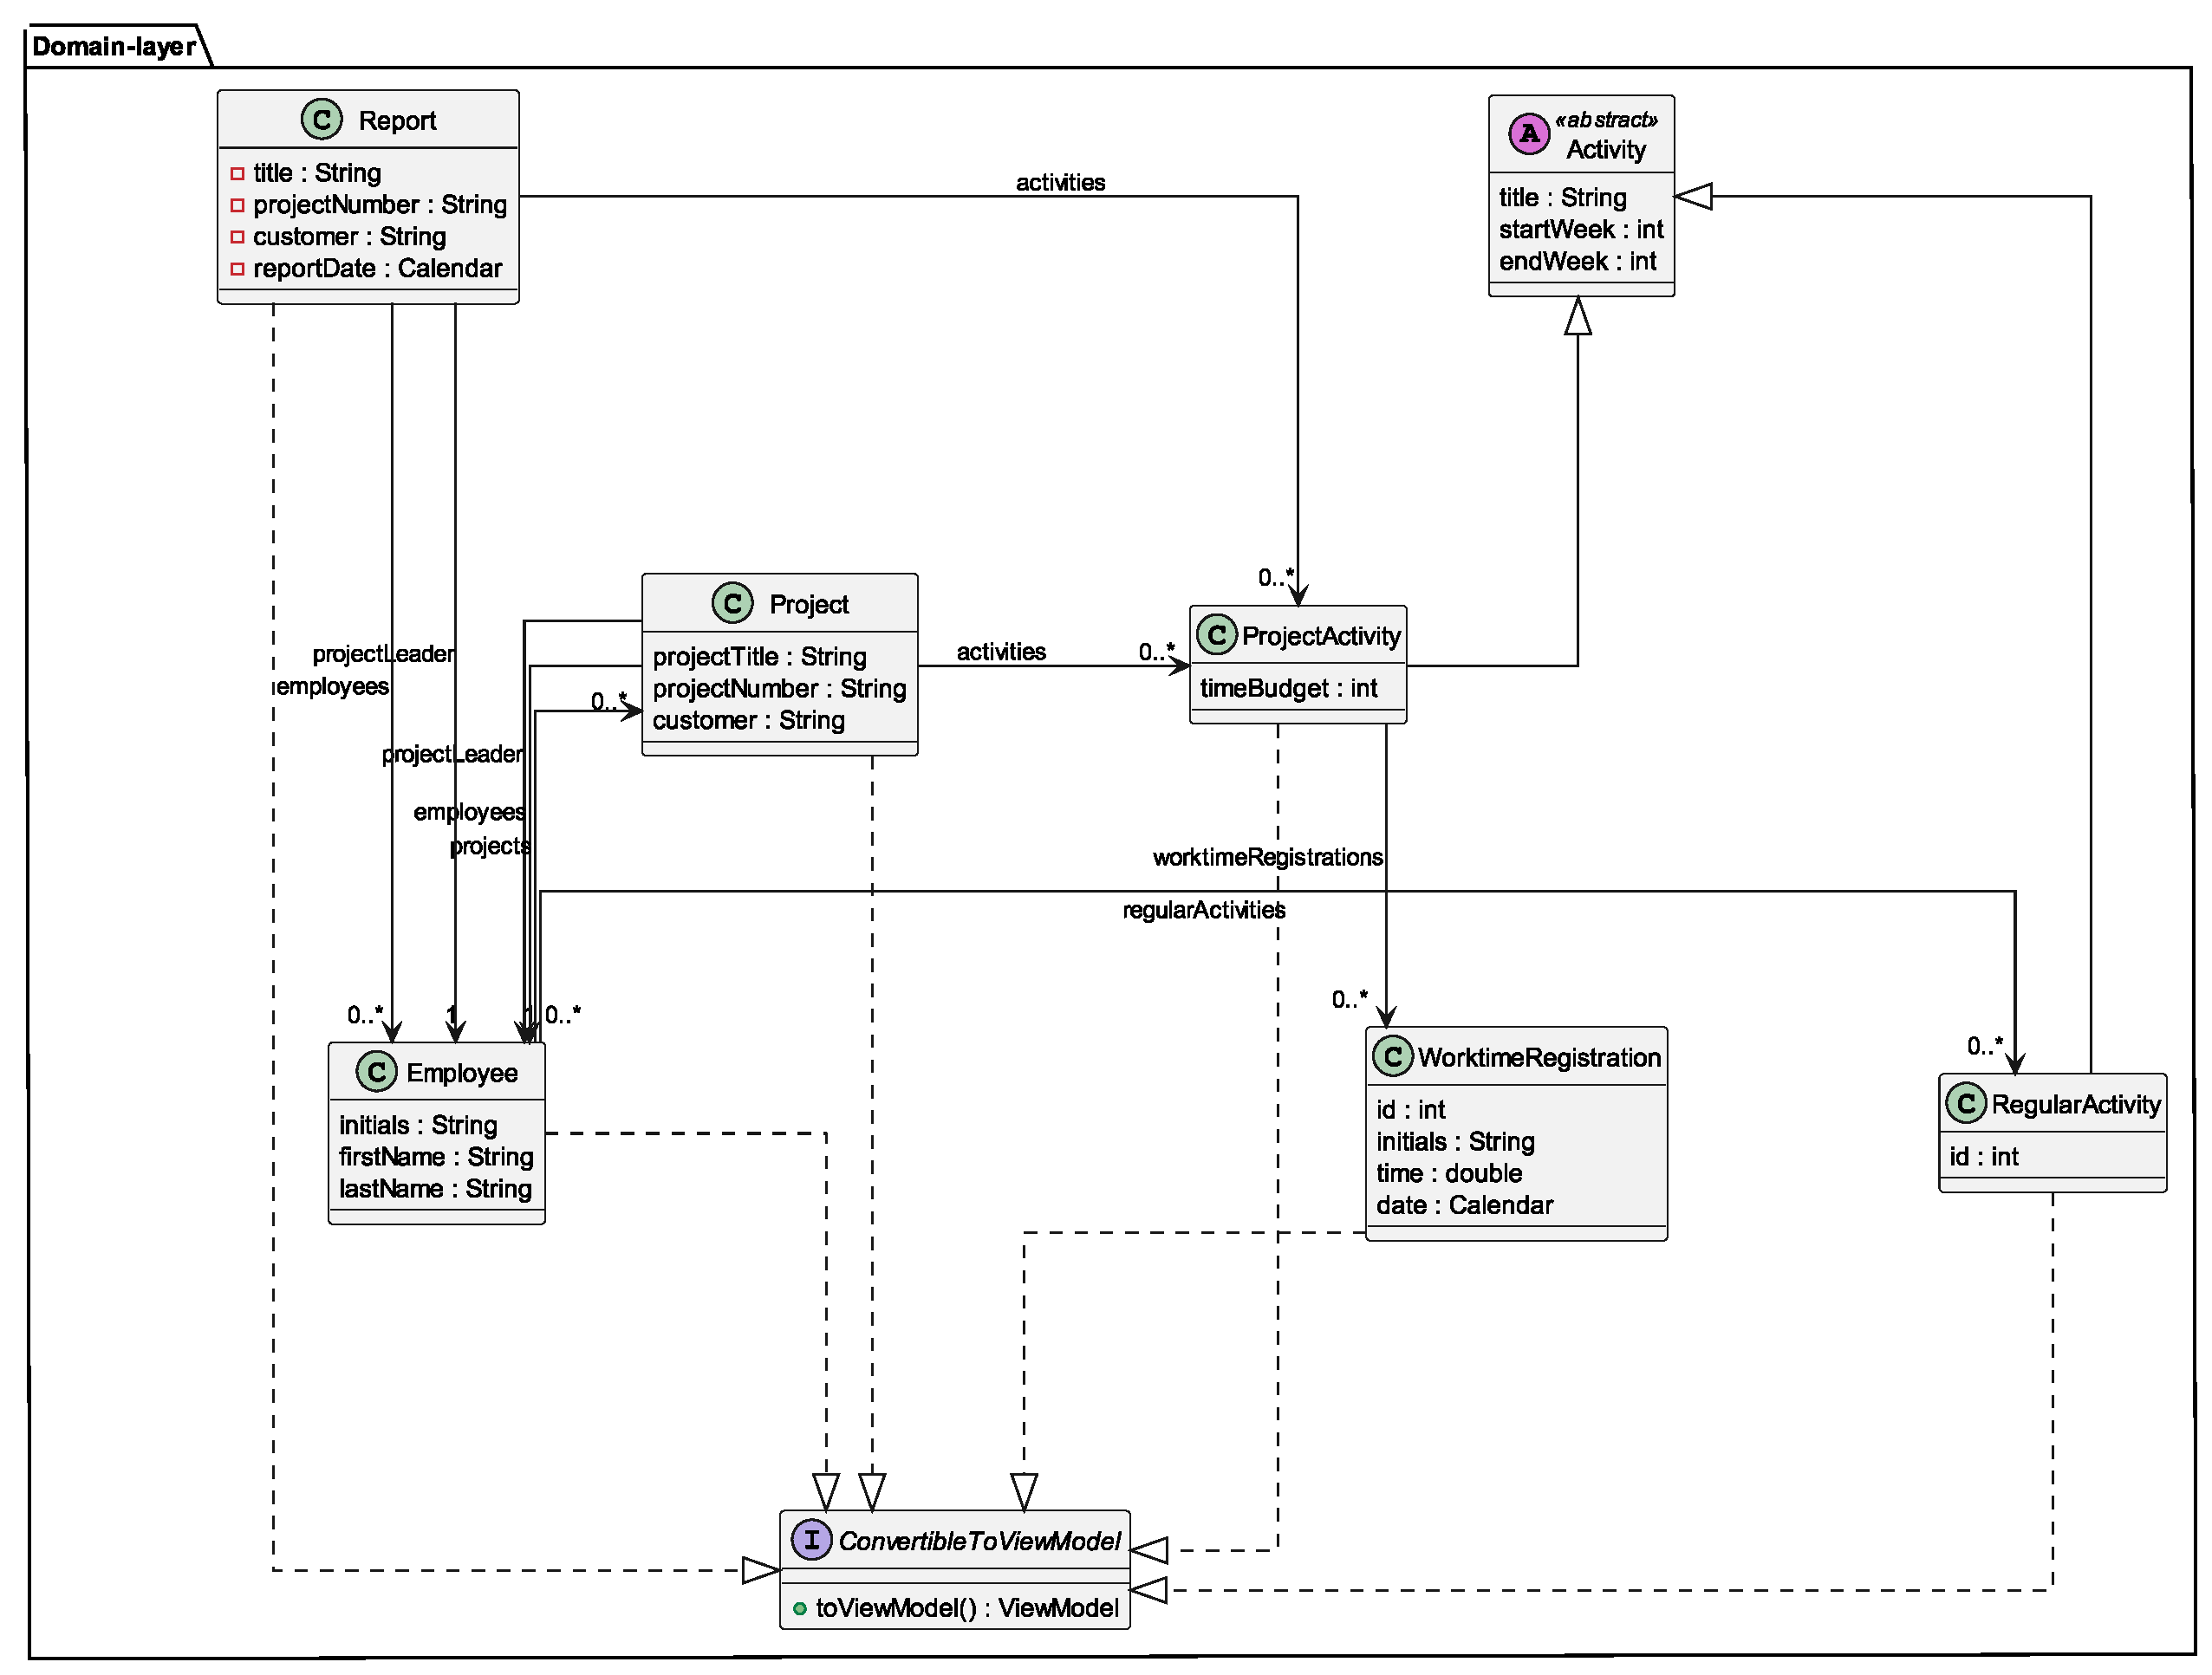
\includegraphics[width=\textwidth]{TaskFusion/out/assets/diagrams/class_persistency_domain/ClassDiagram_domain.eps}
\end{figure}
Skal data bruges i CLI'en hentes en \textit{ModelViewModel} af et objekt, som CLI'en formaterer til brugerfladen.
\newpage
\subsection{Sekvensdiagrammer}\label{sec:sequence}
\begin{figure}[H]
    \centering
    \caption{Sekvensdiagram: Opret medarbejder}\label{fig:sequenceRegisterEmployee}
    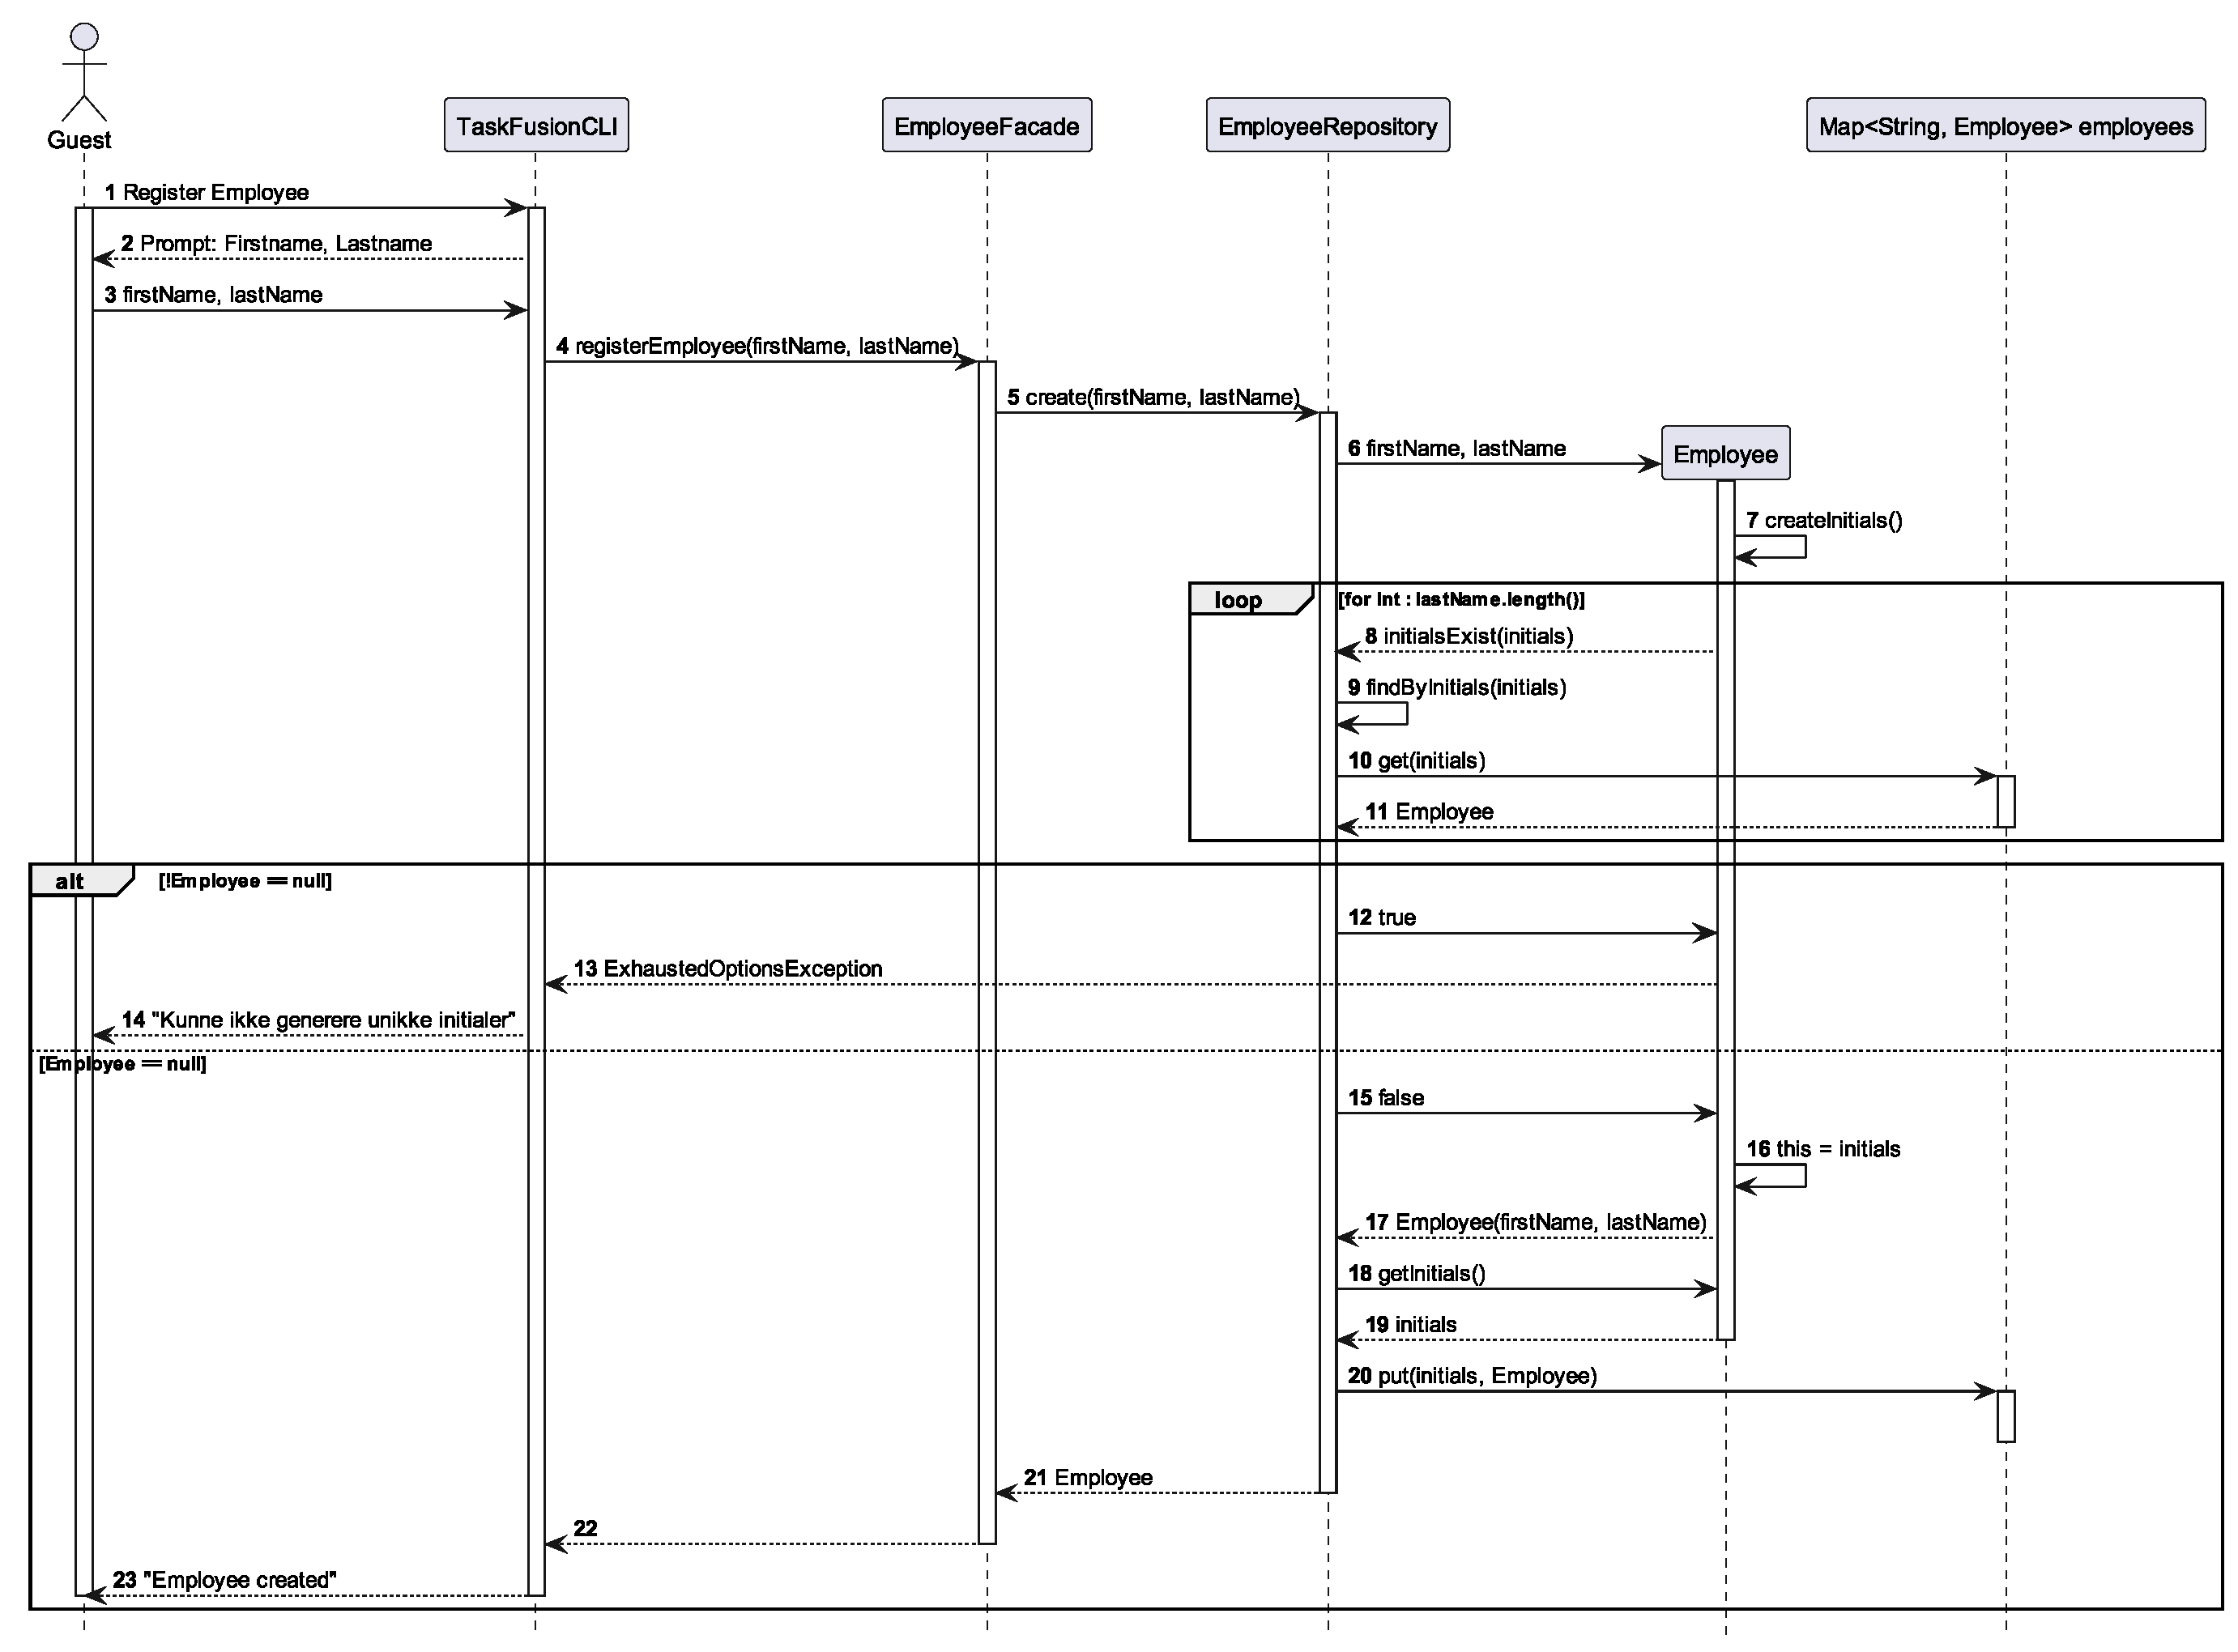
\includegraphics[width=\textwidth]{RequirementsAndDesign/SequenceDiagrams/seqRegisterEmployee.eps}
\end{figure}
\begin{figure}[H]
    \centering
    \caption{Sekvensdiagram: Login}\label{fig:sequenceLogin}
    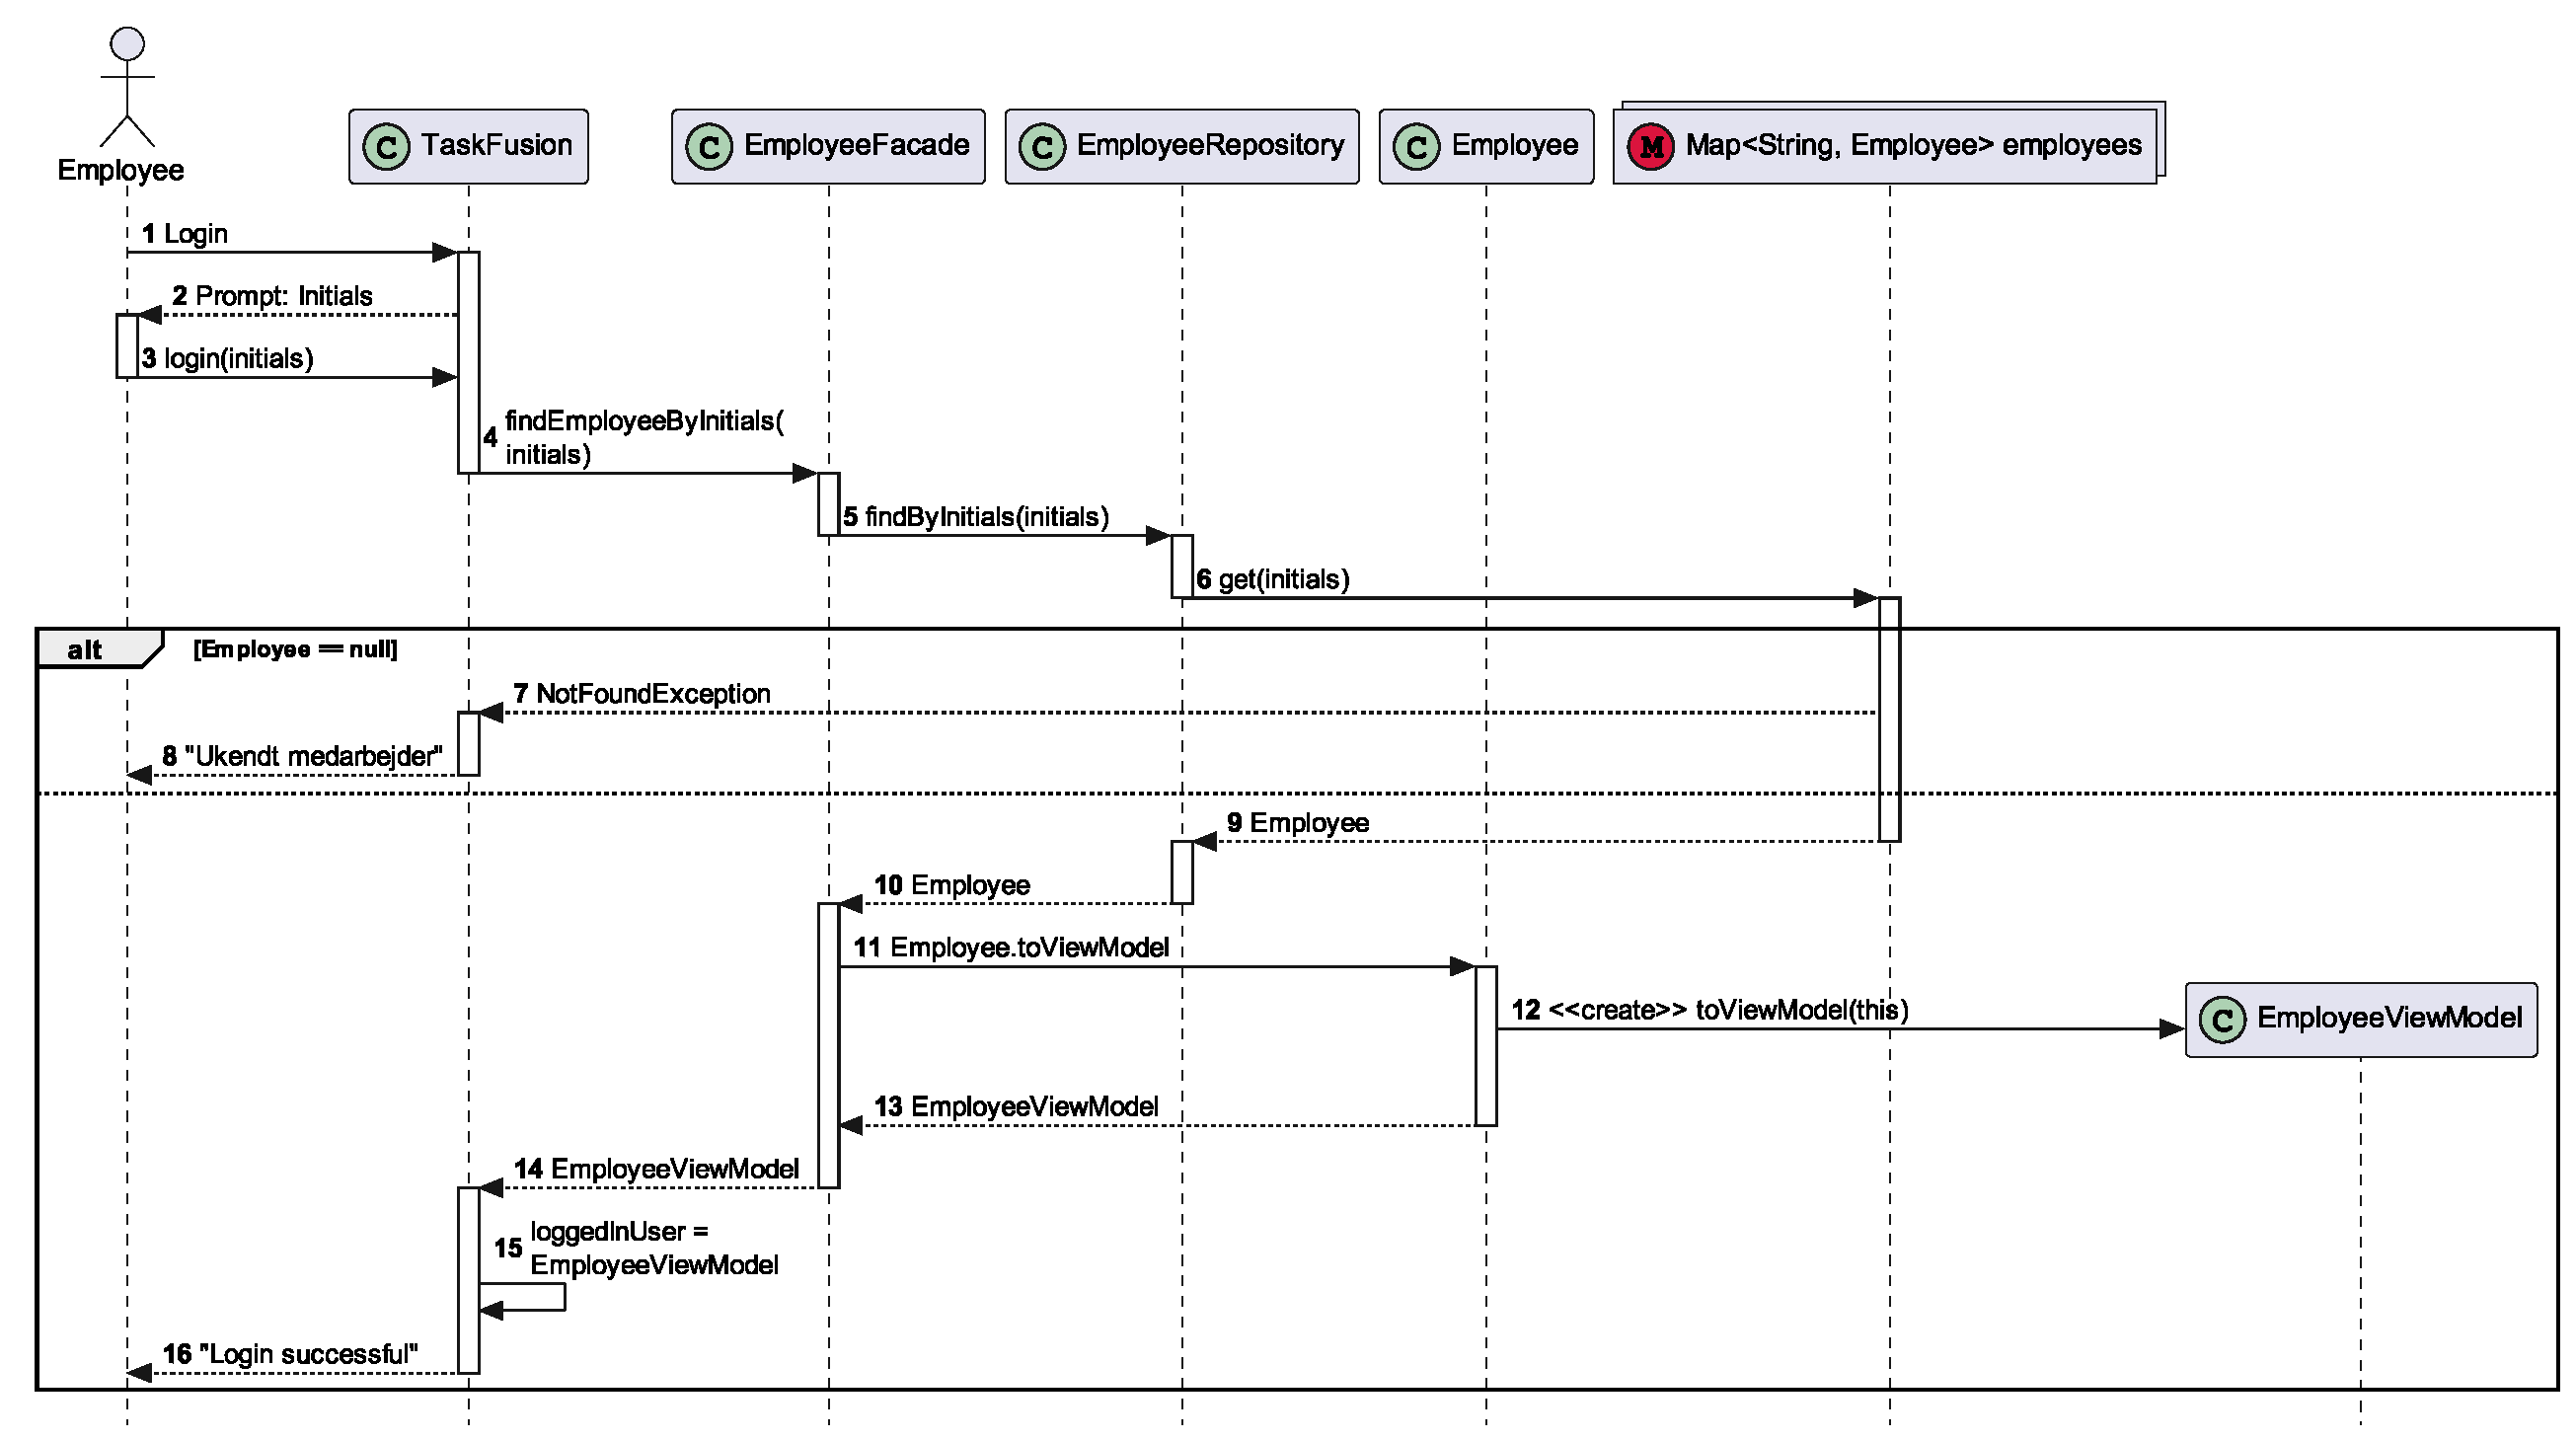
\includegraphics[width=\textwidth]{RequirementsAndDesign/SequenceDiagrams/seqLogin.eps}
\end{figure}
\begin{figure}[H]
    \centering
    \caption{Sekvensdiagram: Logout}\label{fig:sequenceLogout}
    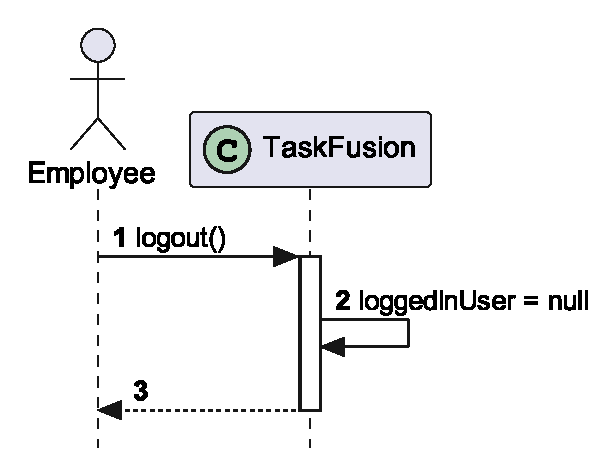
\includegraphics[width=.3\textwidth]{RequirementsAndDesign/SequenceDiagrams/seqLogout.eps}
\end{figure}
\begin{figure}[H]
    \centering
    \caption{Sekvensdiagram: Opret projekt}\label{fig:sequenceCreateProject}
    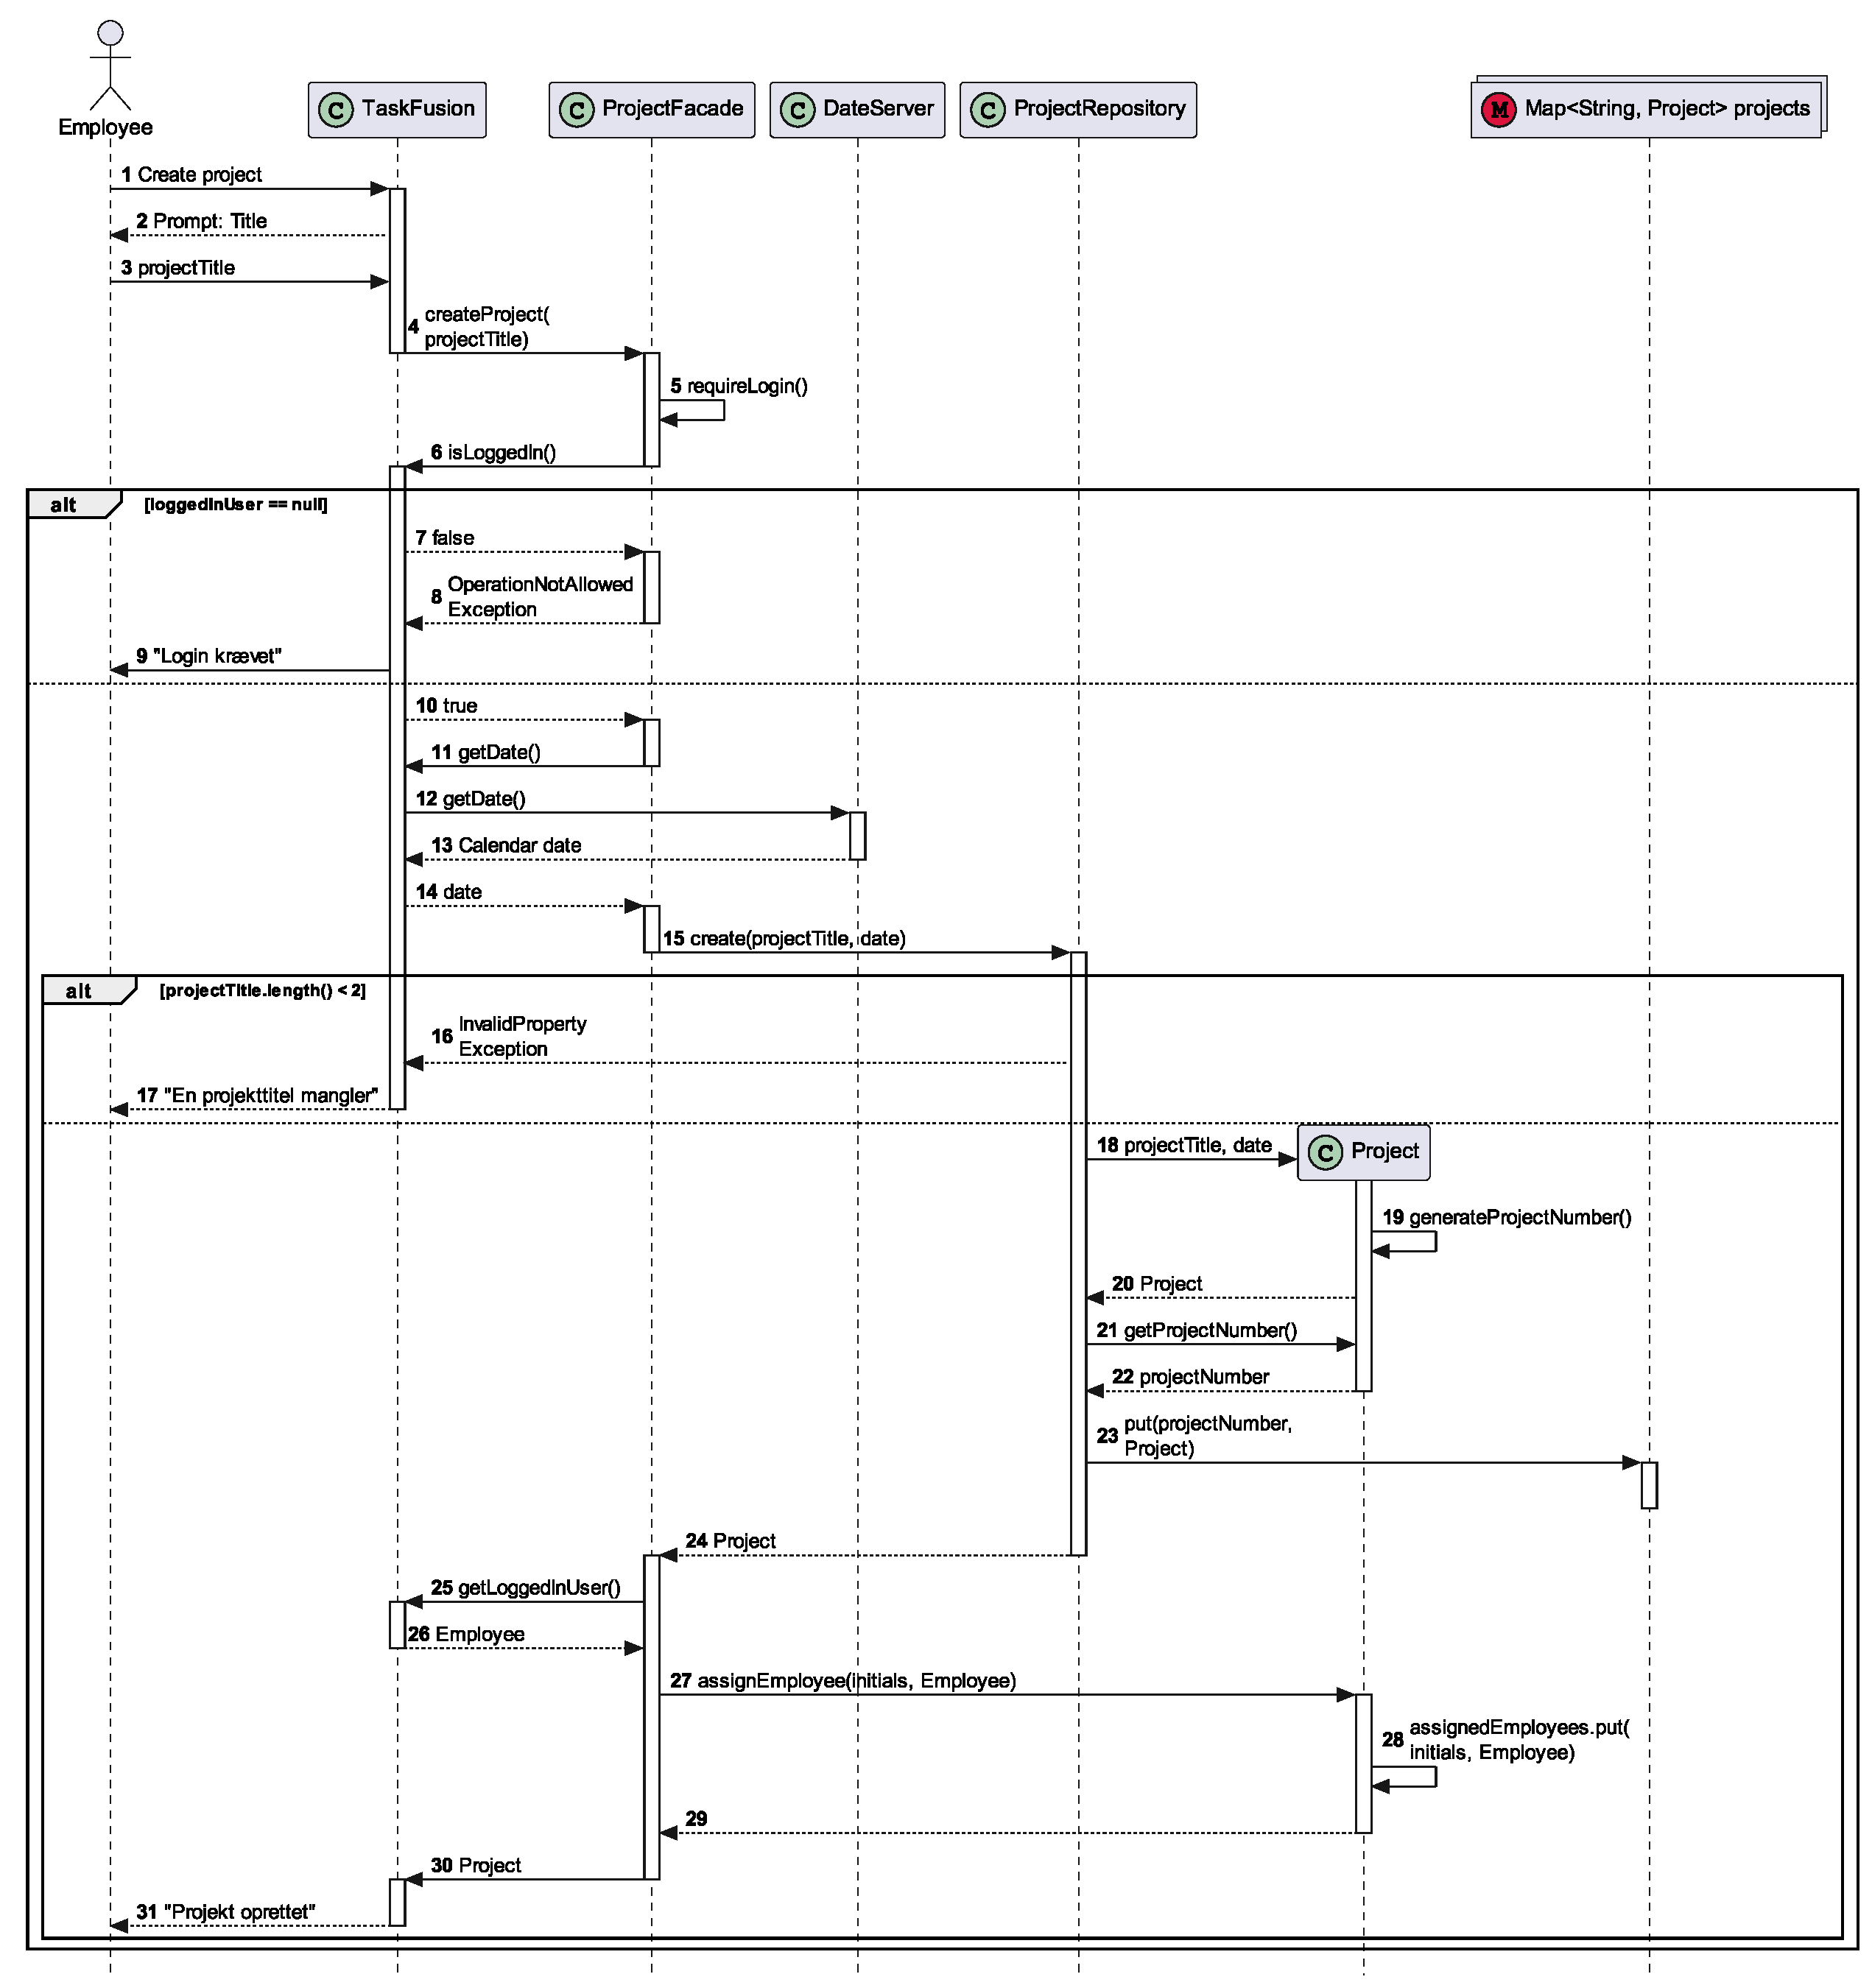
\includegraphics[width=\textwidth]{RequirementsAndDesign/SequenceDiagrams/seqCreateProject.eps}
\end{figure}
\begin{figure}[H]
    \centering
    \caption{Sekvensdiagram: Påtag projektlederrolle}\label{fig:sequenceTakePLRole}
    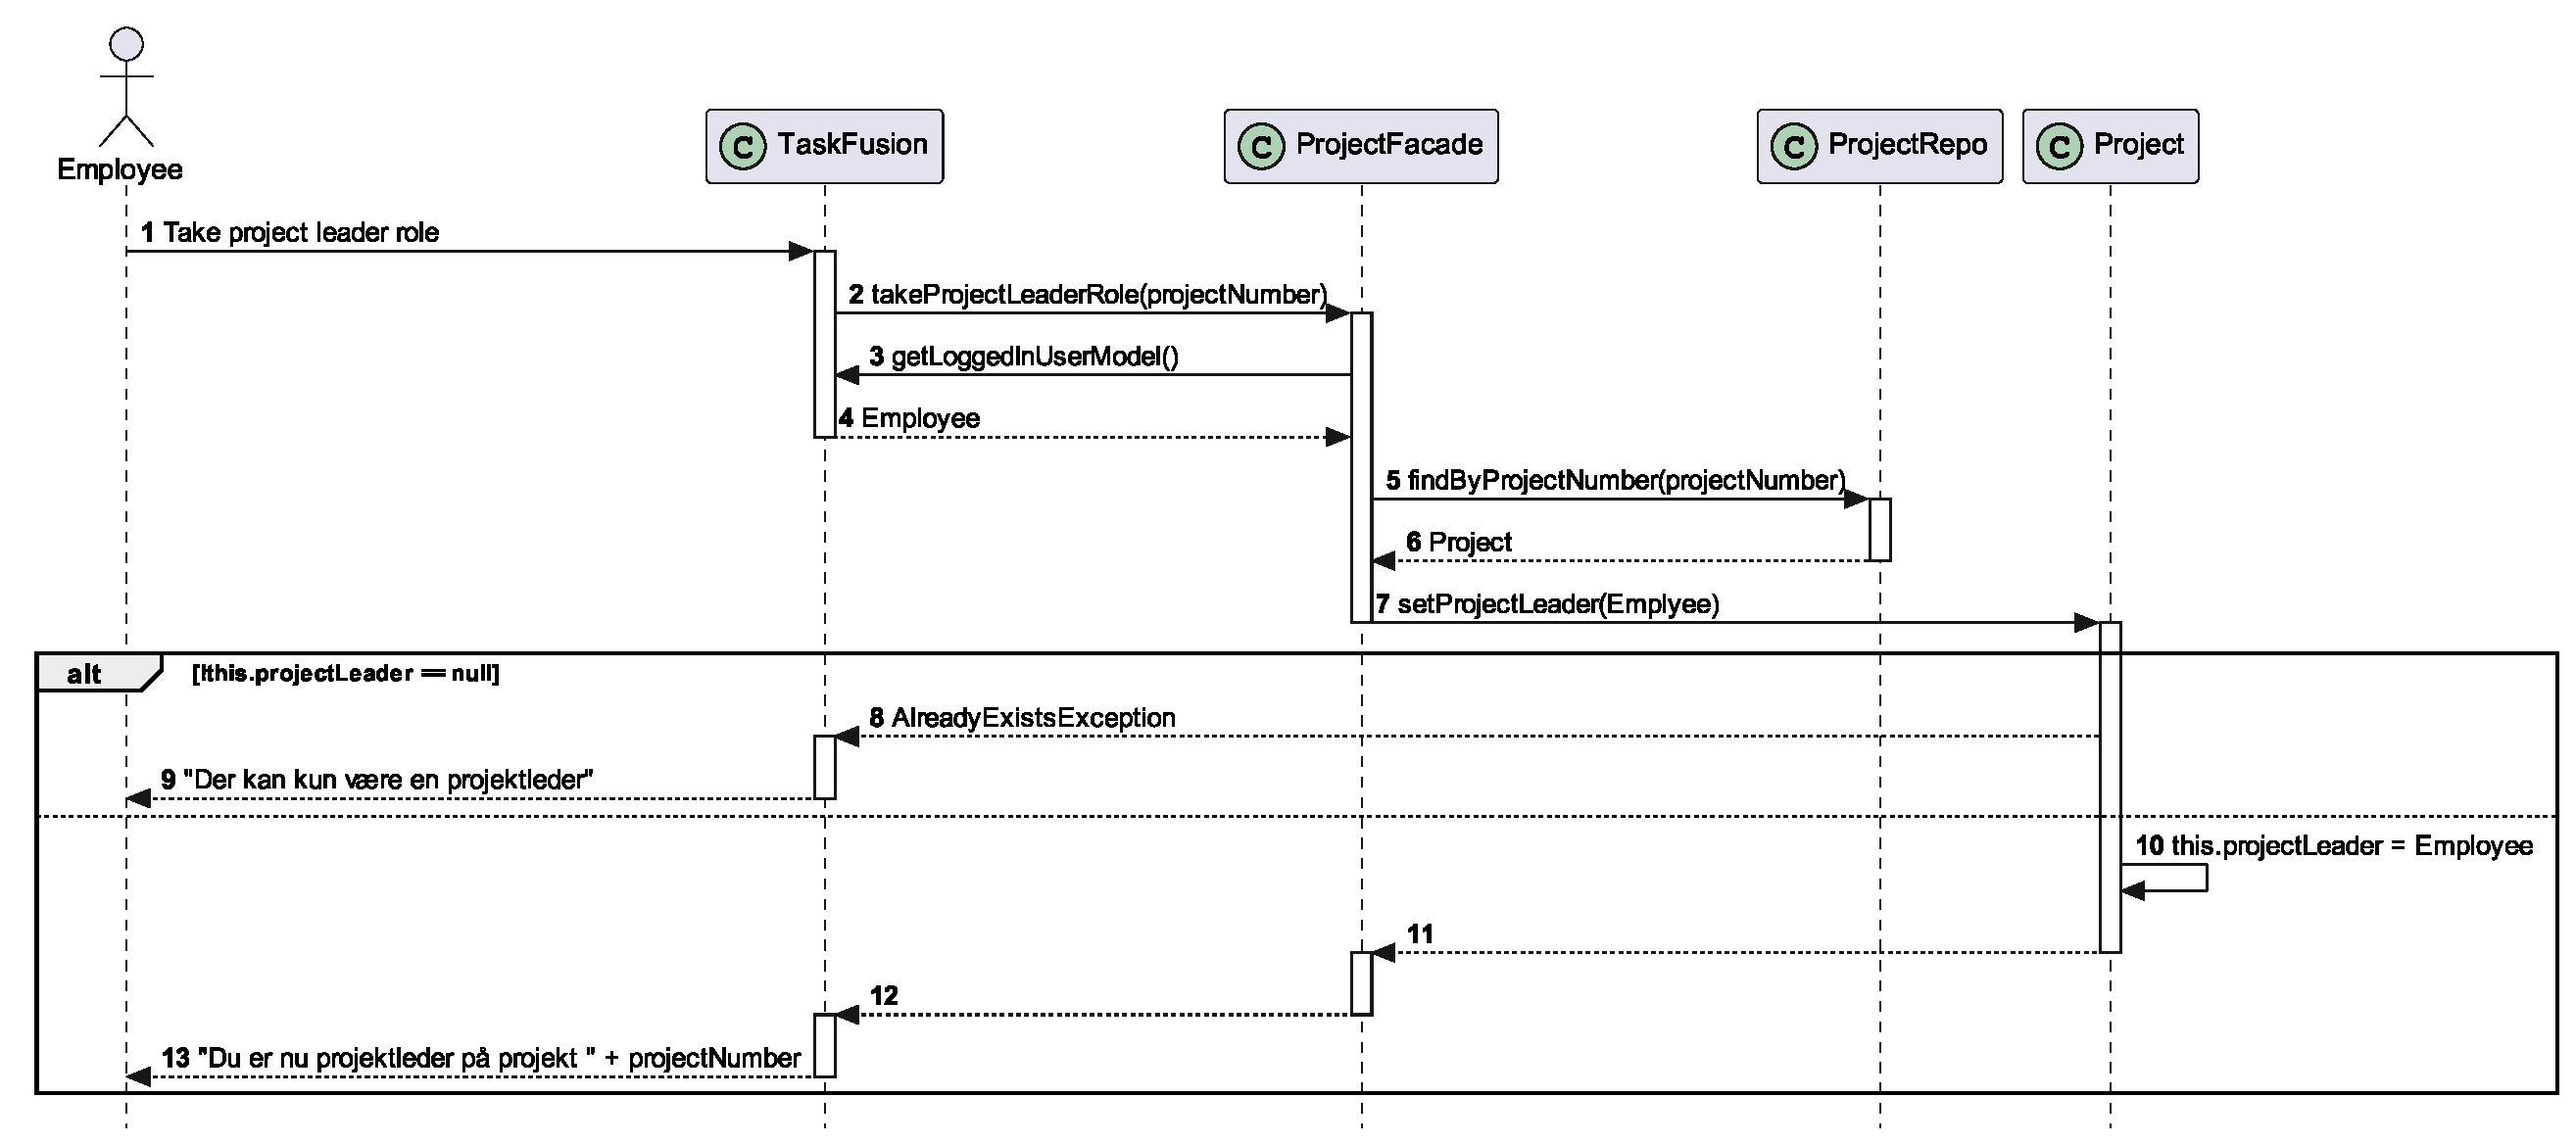
\includegraphics[width=\textwidth]{RequirementsAndDesign/SequenceDiagrams/seqTakePLRole.eps}
\end{figure}
\begin{figure}[H]
    \centering
    \caption{Sekvensdiagram: Tildel medarbejder til projekt}\label{fig:sequenceAssignEmployee}
    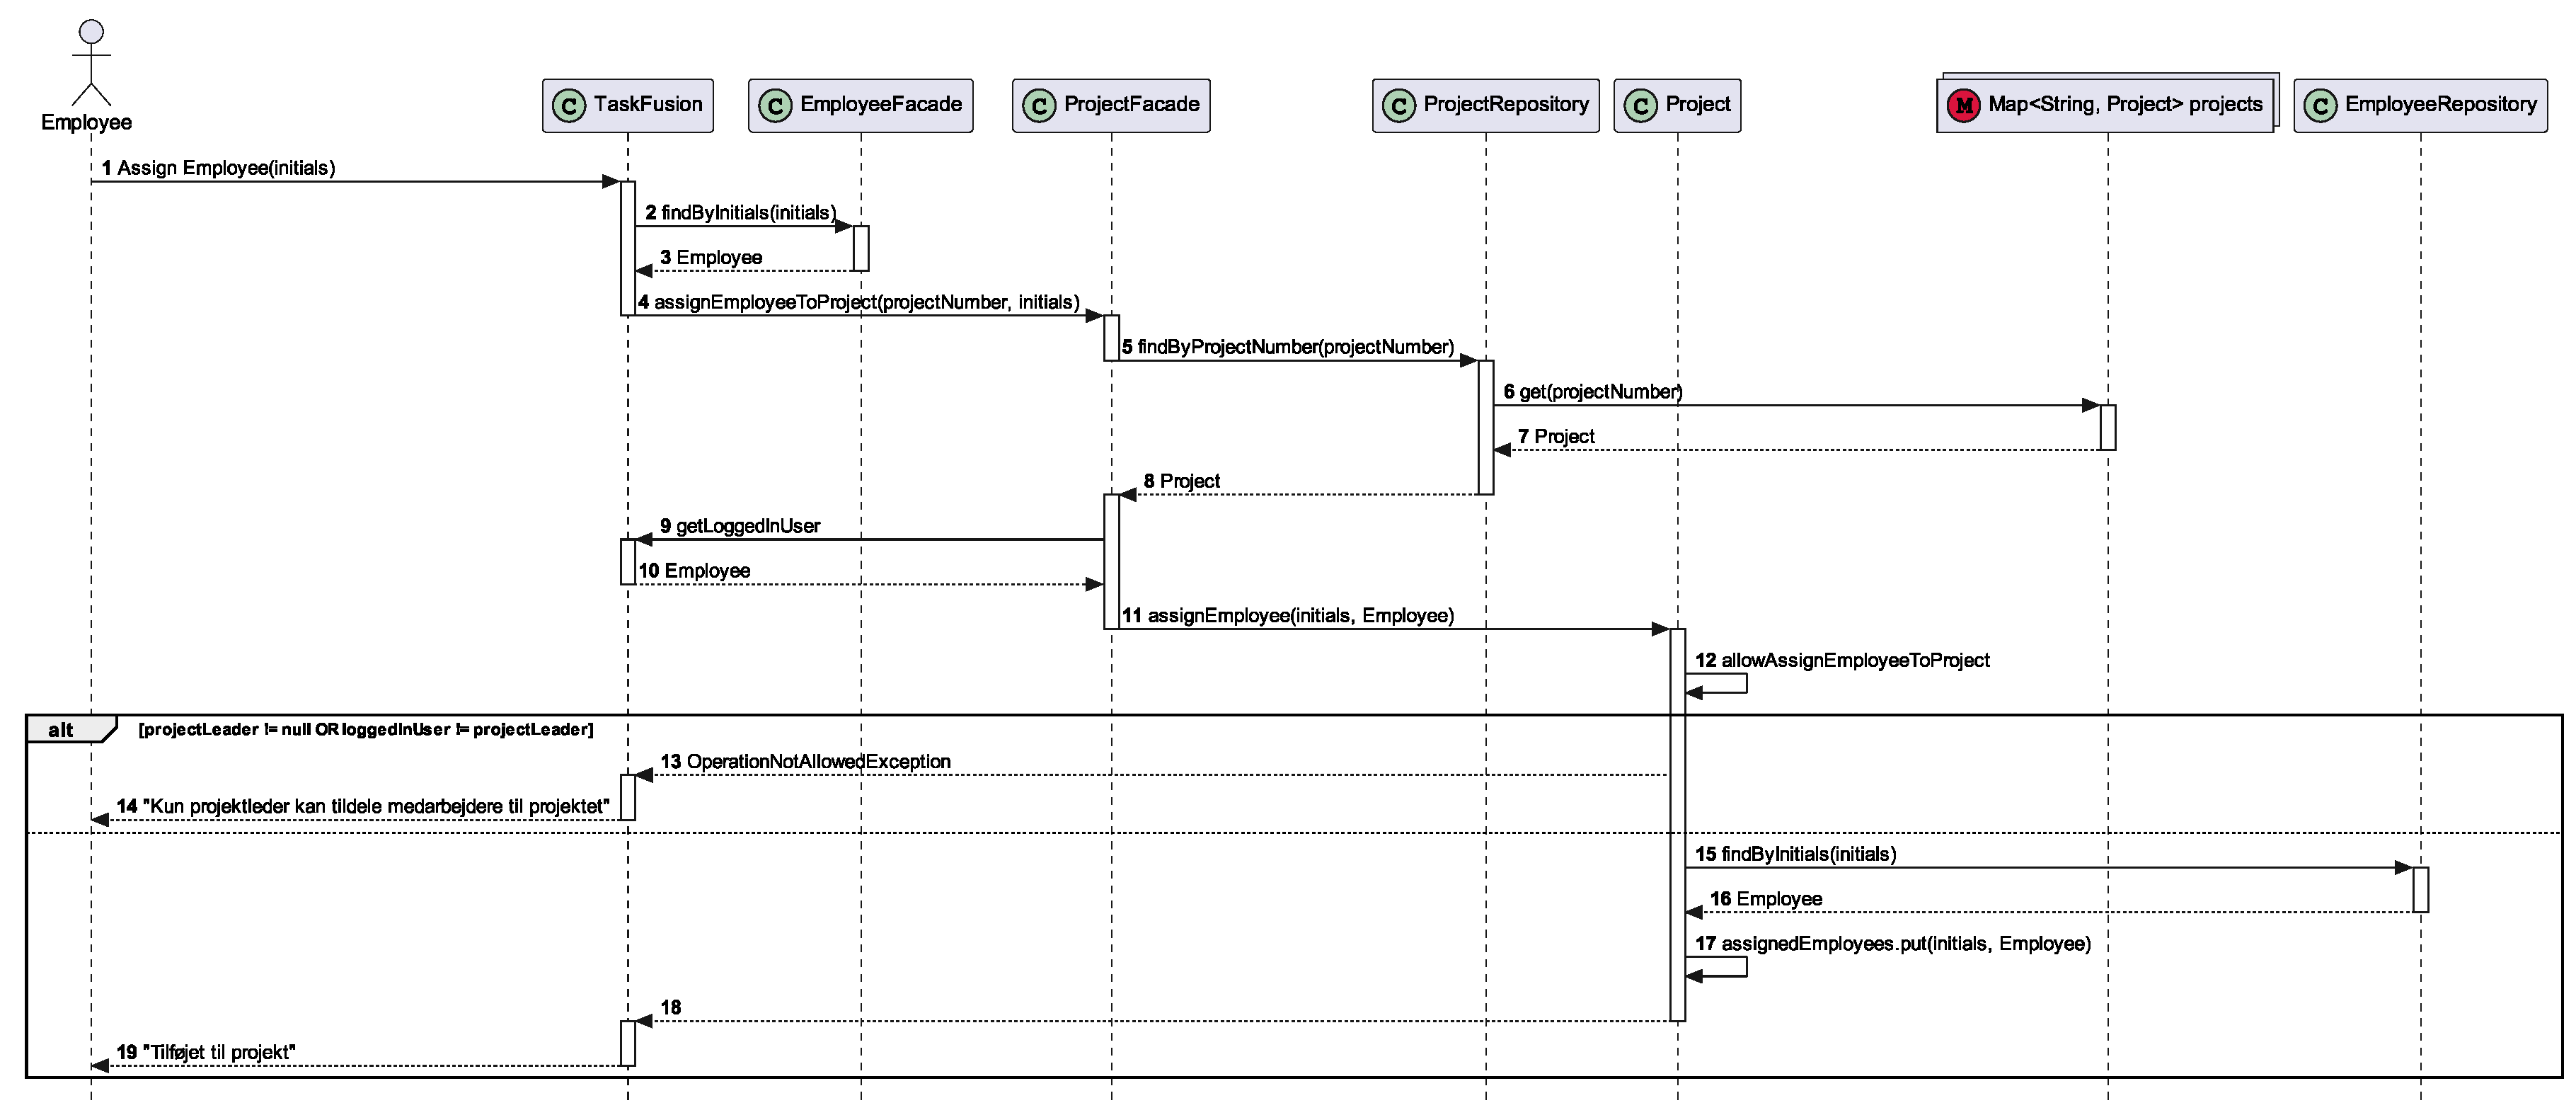
\includegraphics[width=\textwidth]{RequirementsAndDesign/SequenceDiagrams/seqAssignEmployee.eps}
\end{figure}
\begin{figure}[H]
    \centering
    \caption{Sekvensdiagram: Se medarbejdere tilknyttet et projekt}\label{fig:ViewAssignedEmployee}
    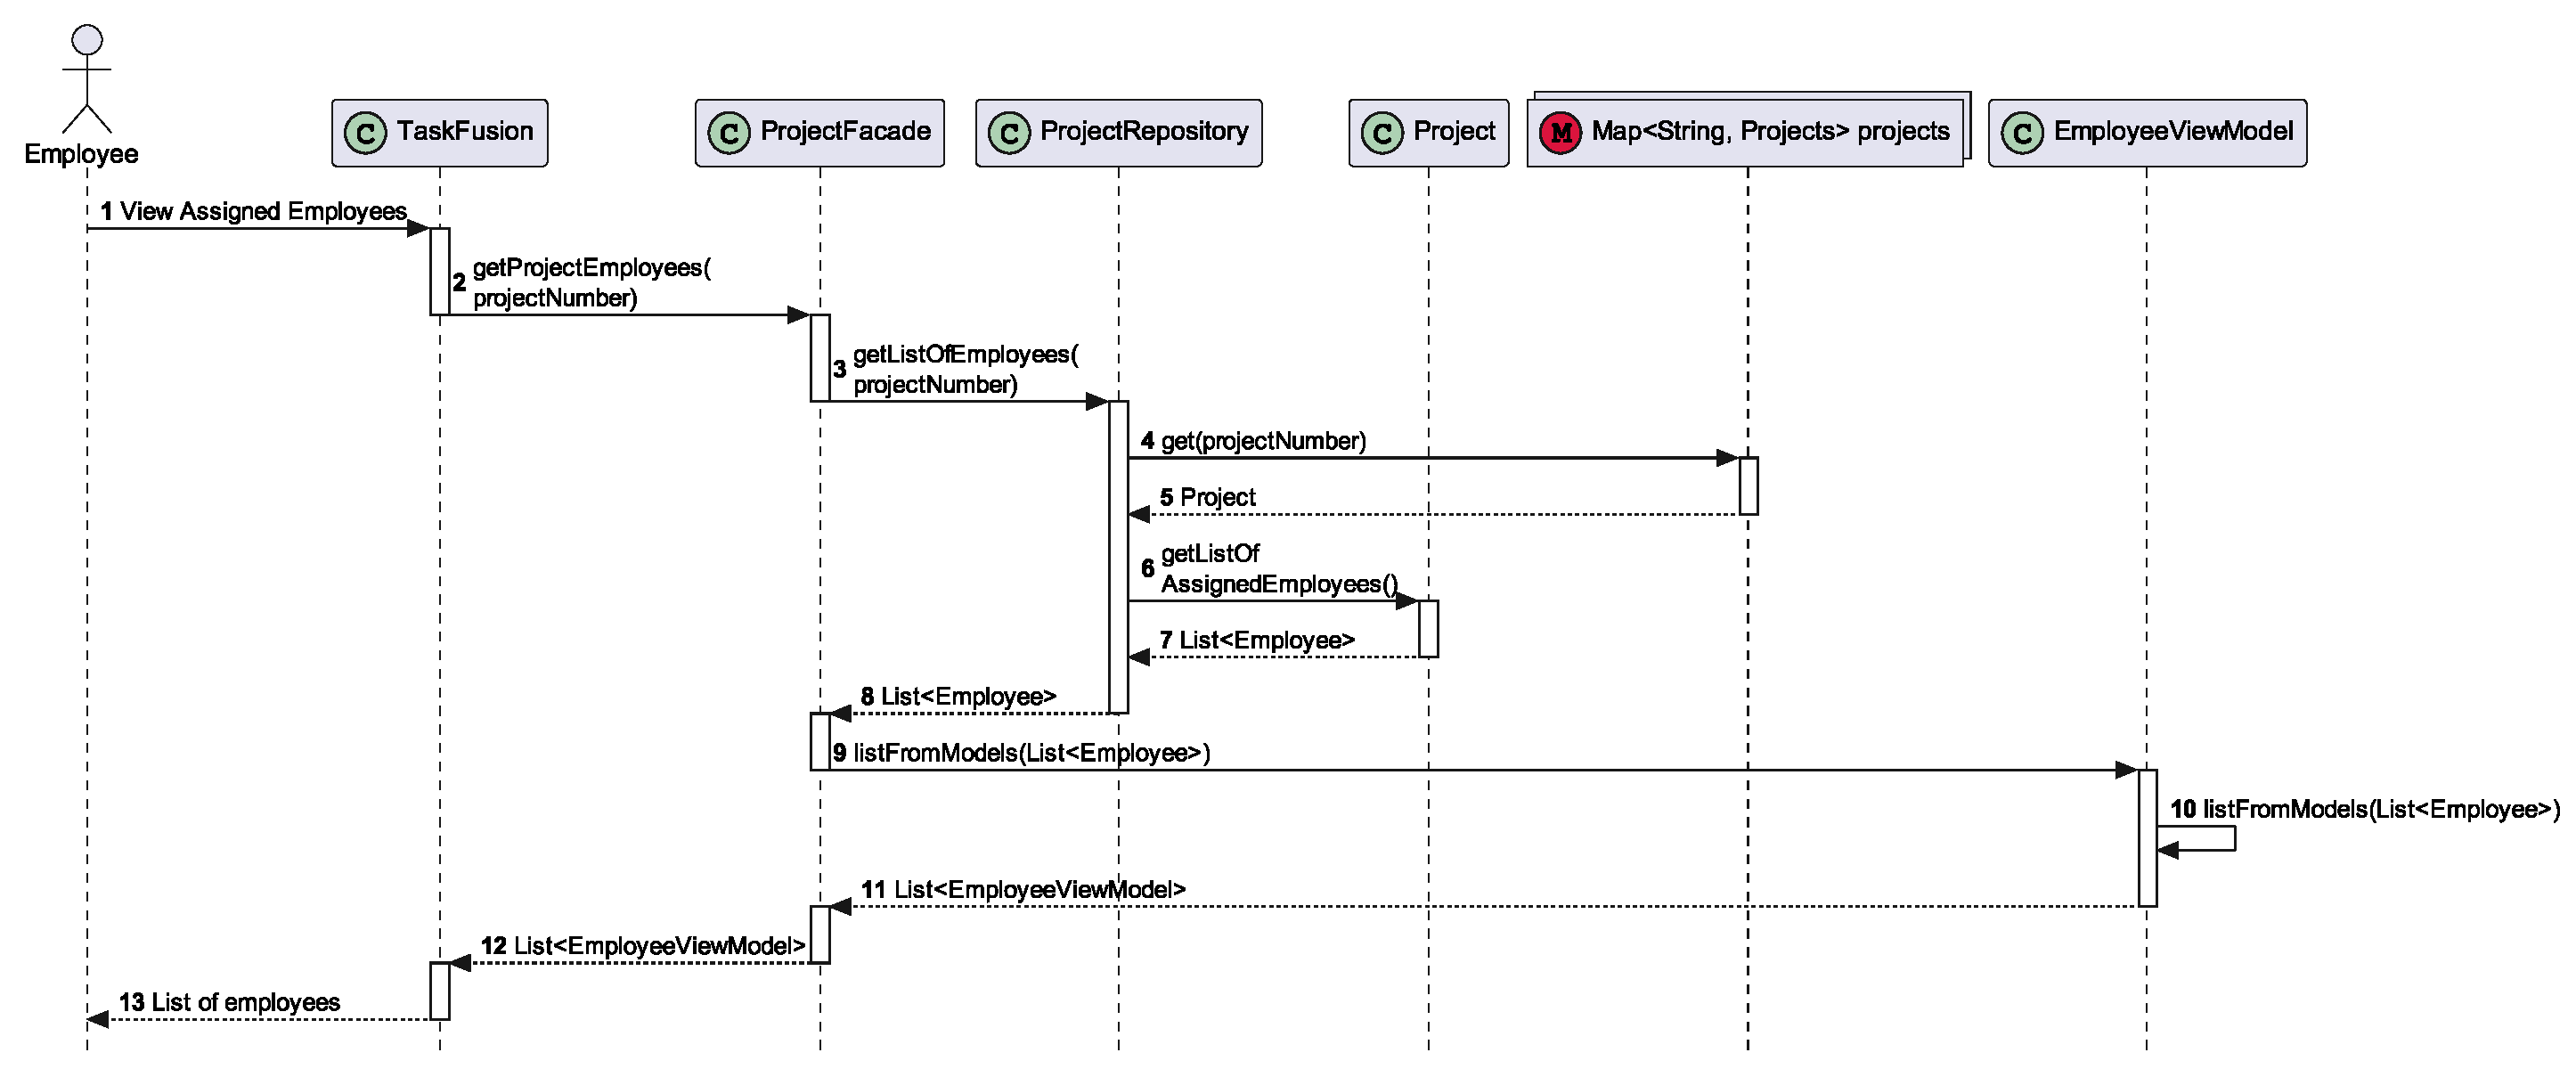
\includegraphics[width=\textwidth]{RequirementsAndDesign/SequenceDiagrams/seqViewAssignedEmployees.eps}
\end{figure}
\begin{figure}[H]
    \centering
    \caption{Sekvensdiagram: Opret projektaktivitet}\label{fig:sequenceCreateProjectActivity}
    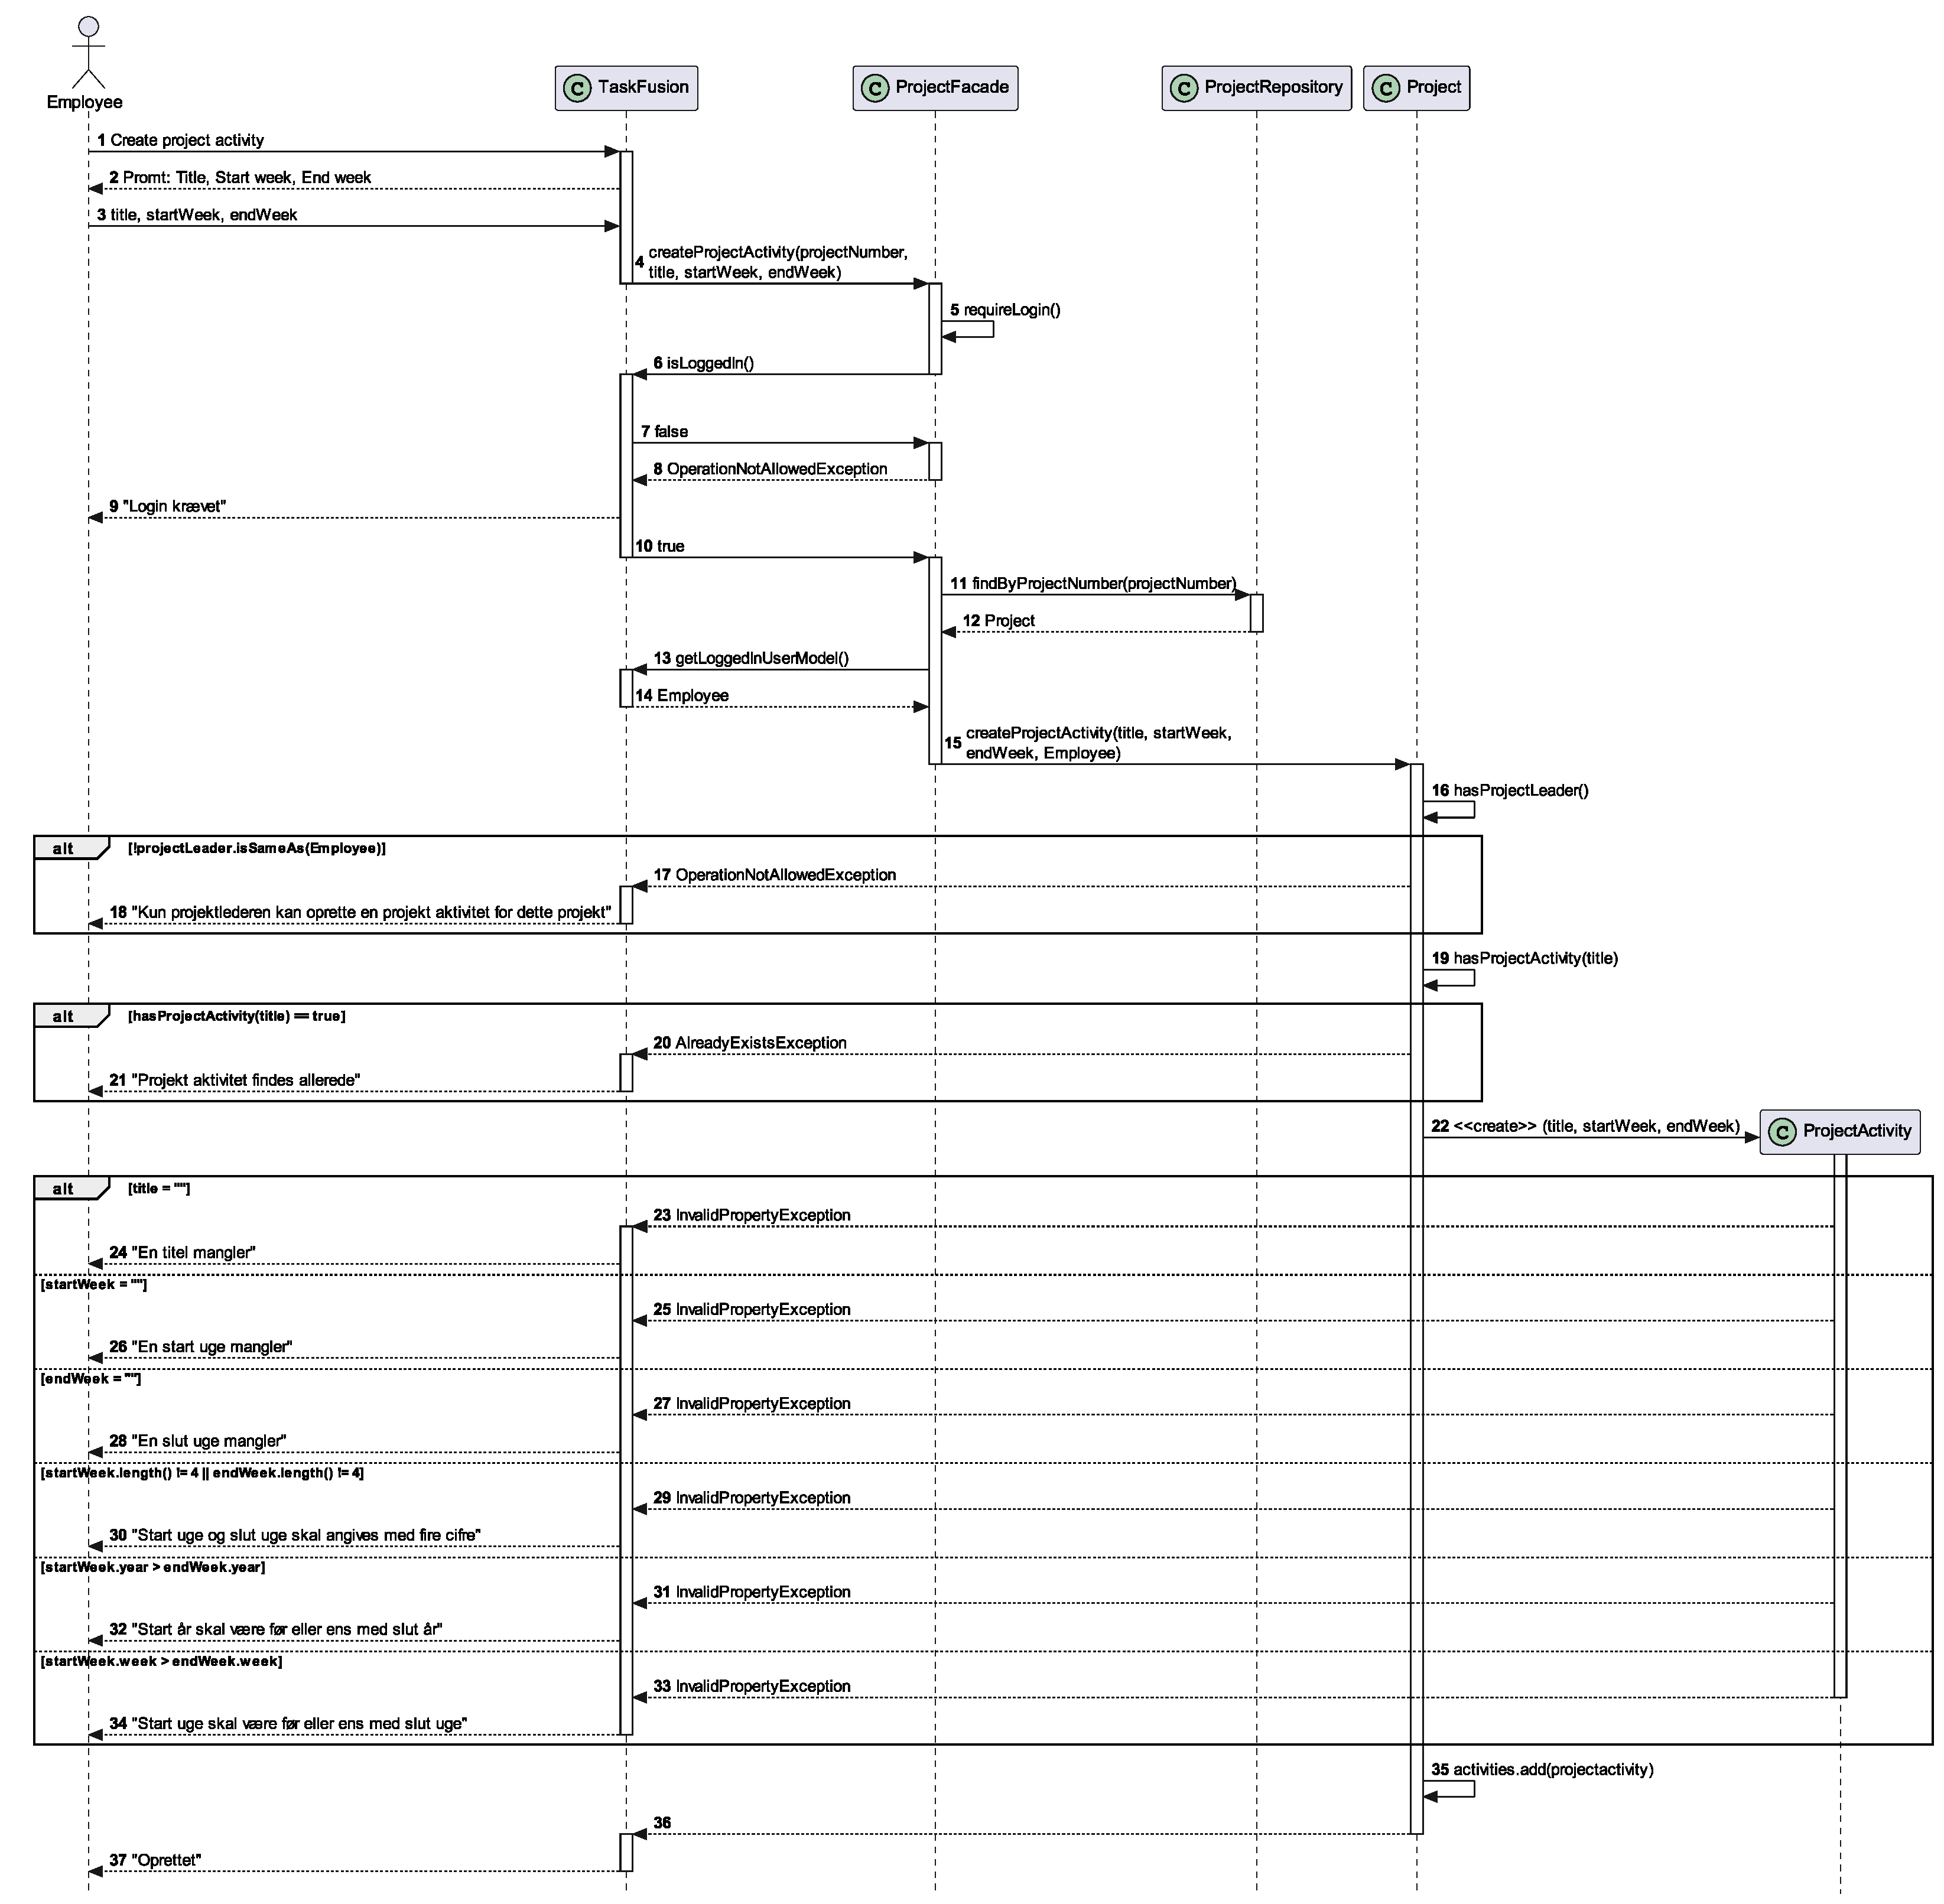
\includegraphics[width=\textwidth]{RequirementsAndDesign/SequenceDiagrams/seqCreateProjectActivity.eps}
\end{figure}
\begin{figure}[H]
    \centering
    \caption{Sekvensdiagram: Anfør tidsbudget på projektaktivitet}\label{fig:sequenceSetTimeBudget}
    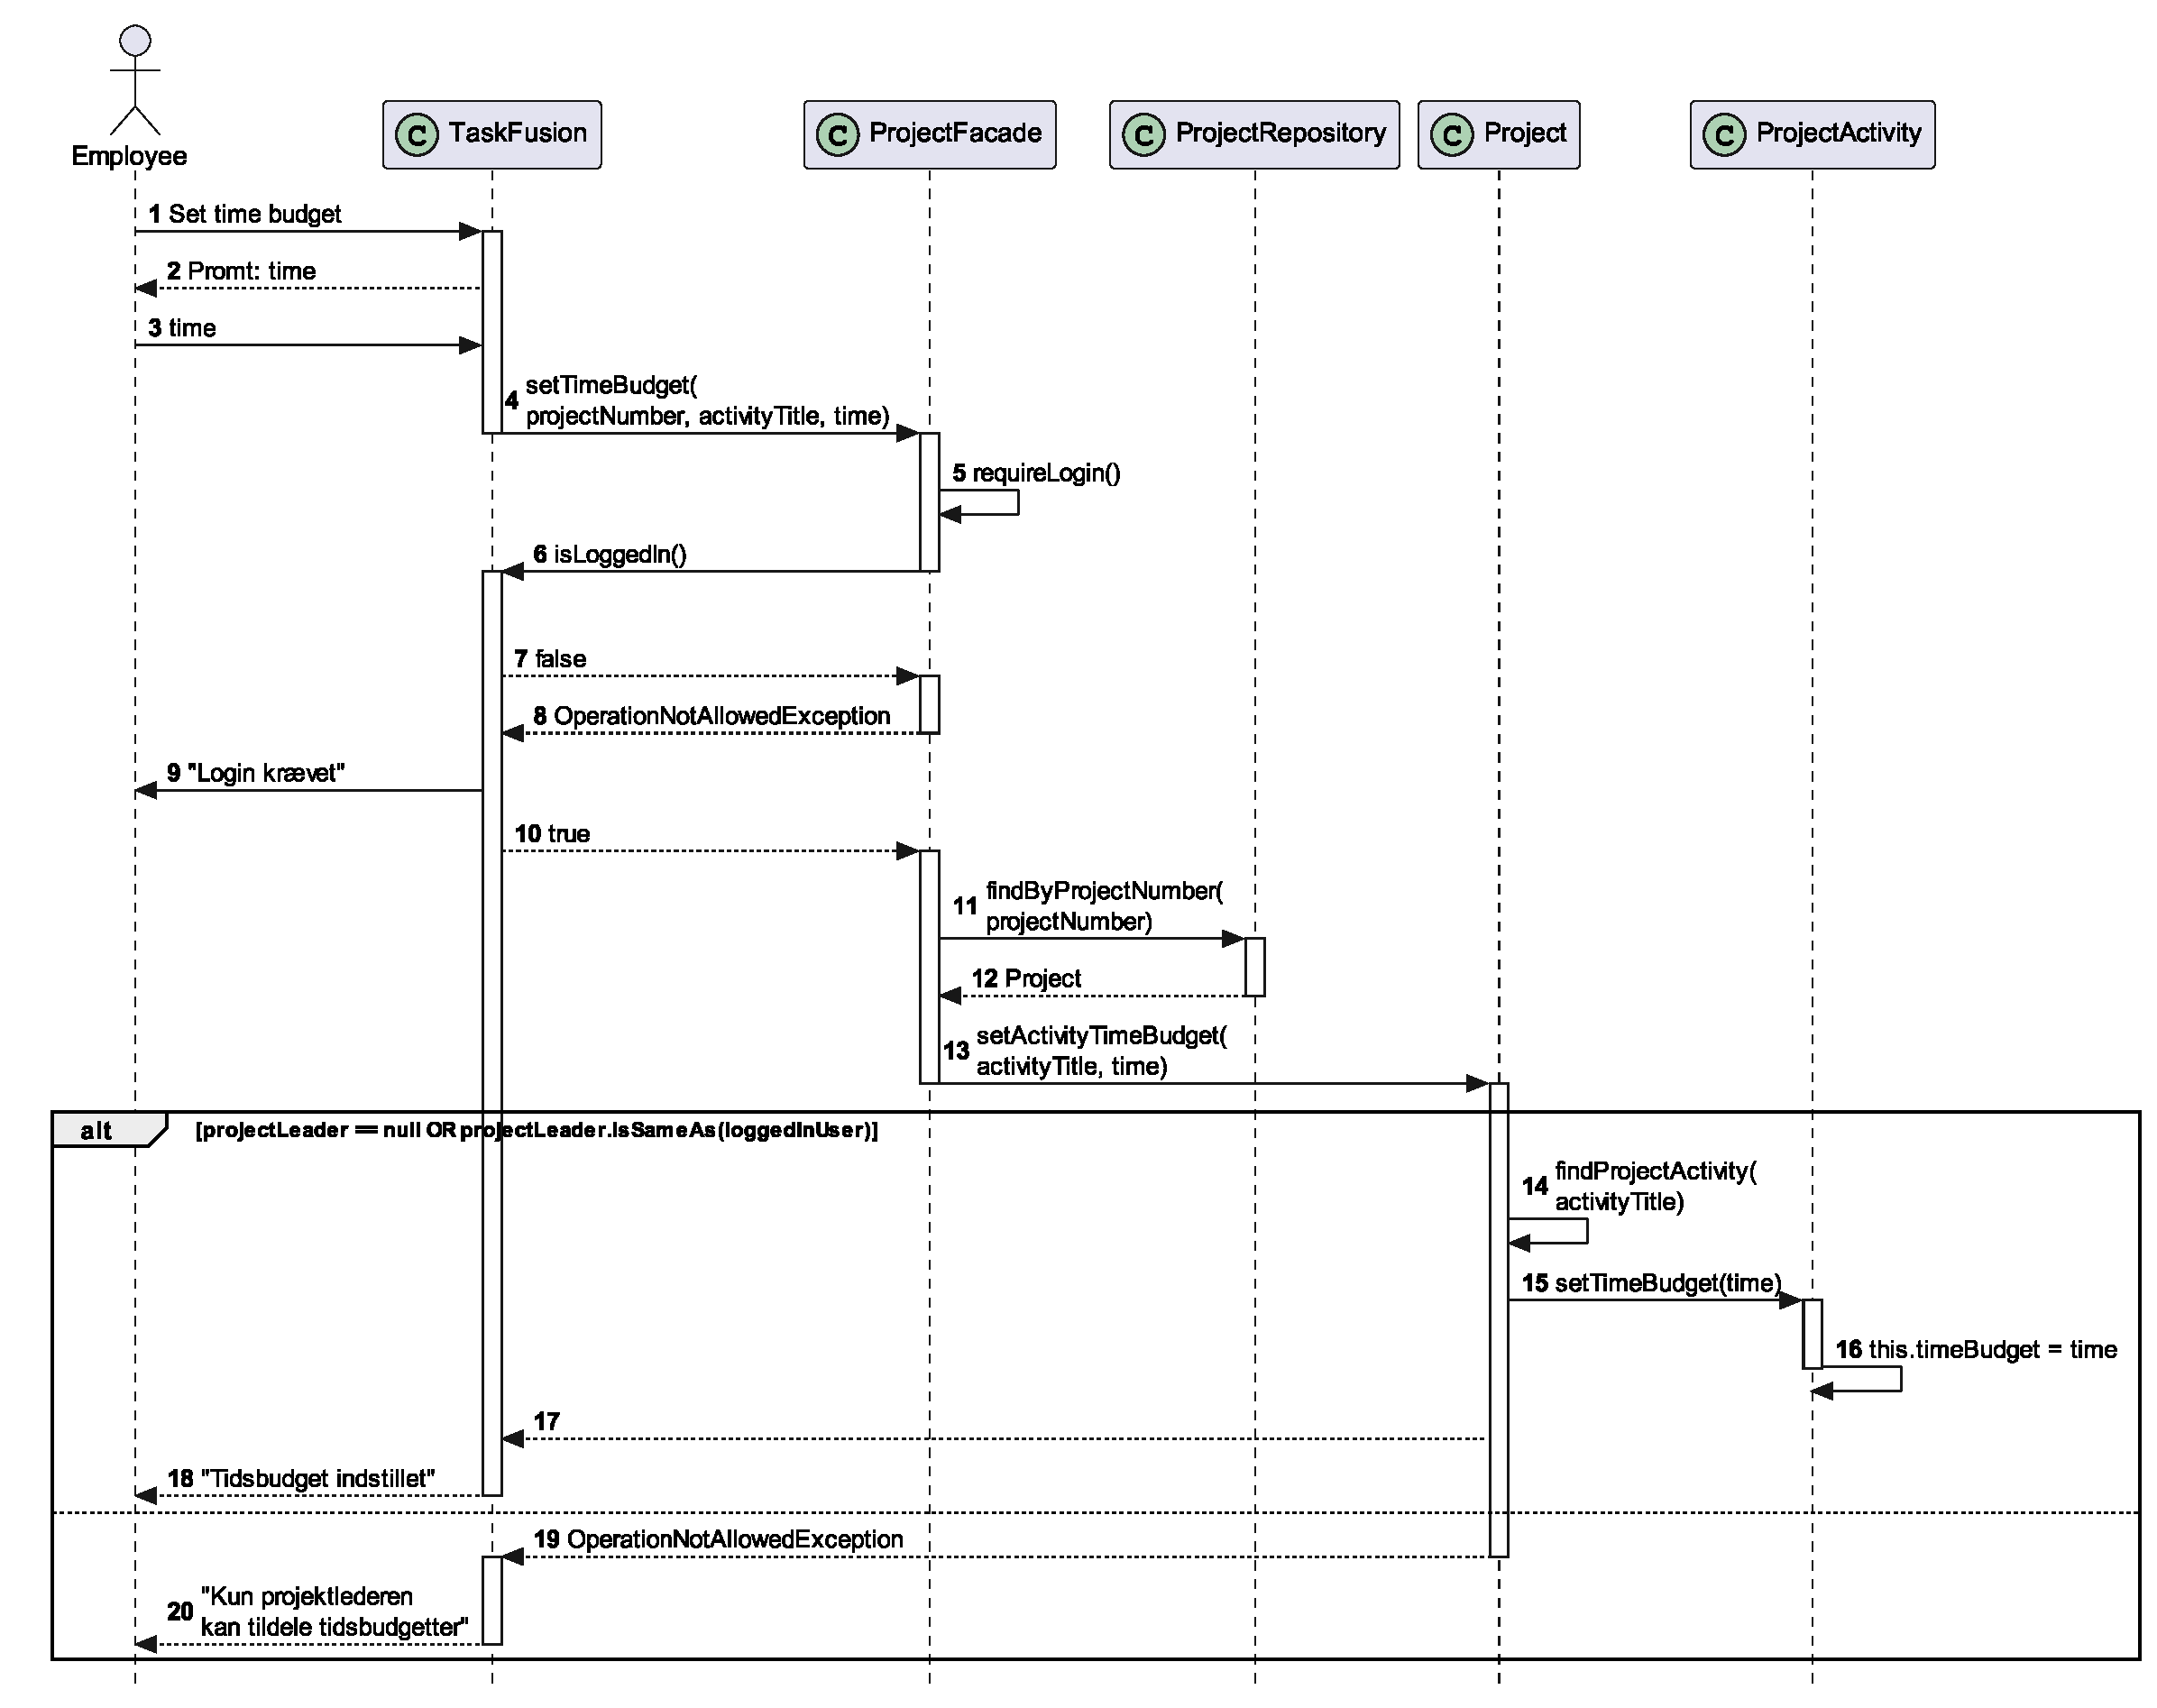
\includegraphics[width=\textwidth]{RequirementsAndDesign/SequenceDiagrams/seqSetTimeBudget.eps}
\end{figure}
\begin{figure}[H]
    \centering
    \caption{Sekvensdiagram: Opret fast aktivitet}\label{fig:sequenceCreateRegularActivity}
    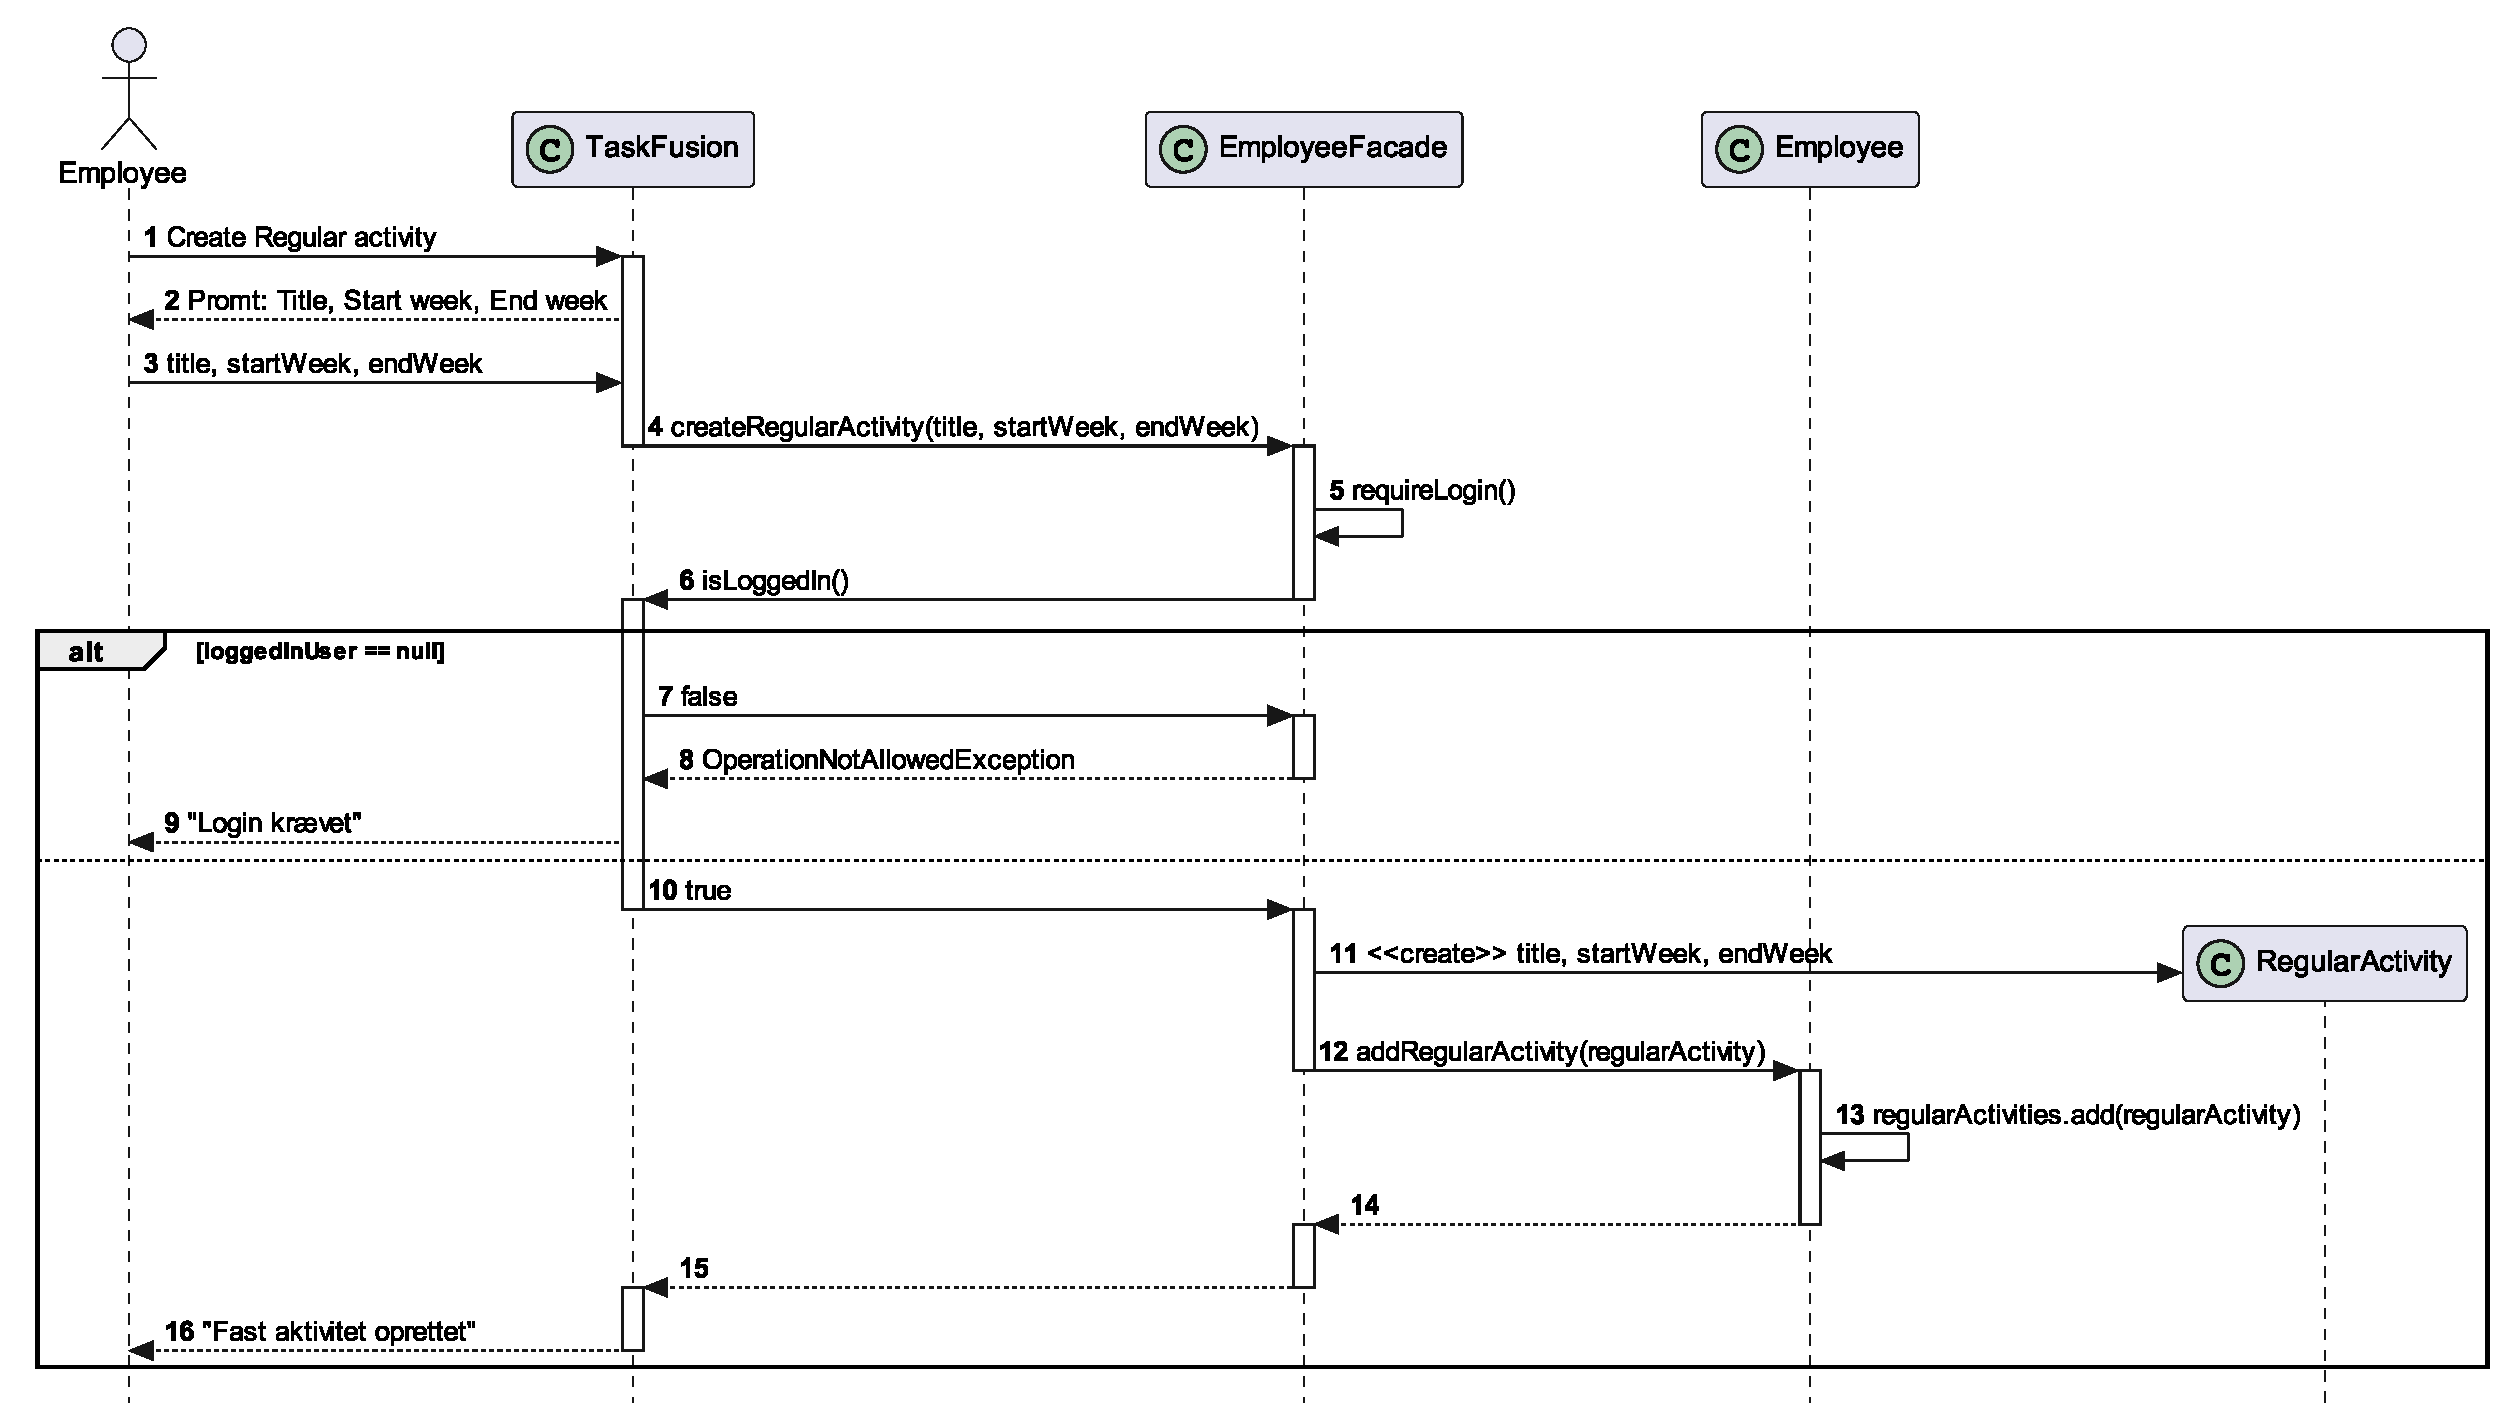
\includegraphics[width=\textwidth]{RequirementsAndDesign/SequenceDiagrams/seqCreateRegularActivity.eps}
\end{figure}
\begin{figure}[H]
    \centering
    \caption{Sekvensdiagram: Se fast aktivitet}\label{fig:sequenceViewRegularActivity}
    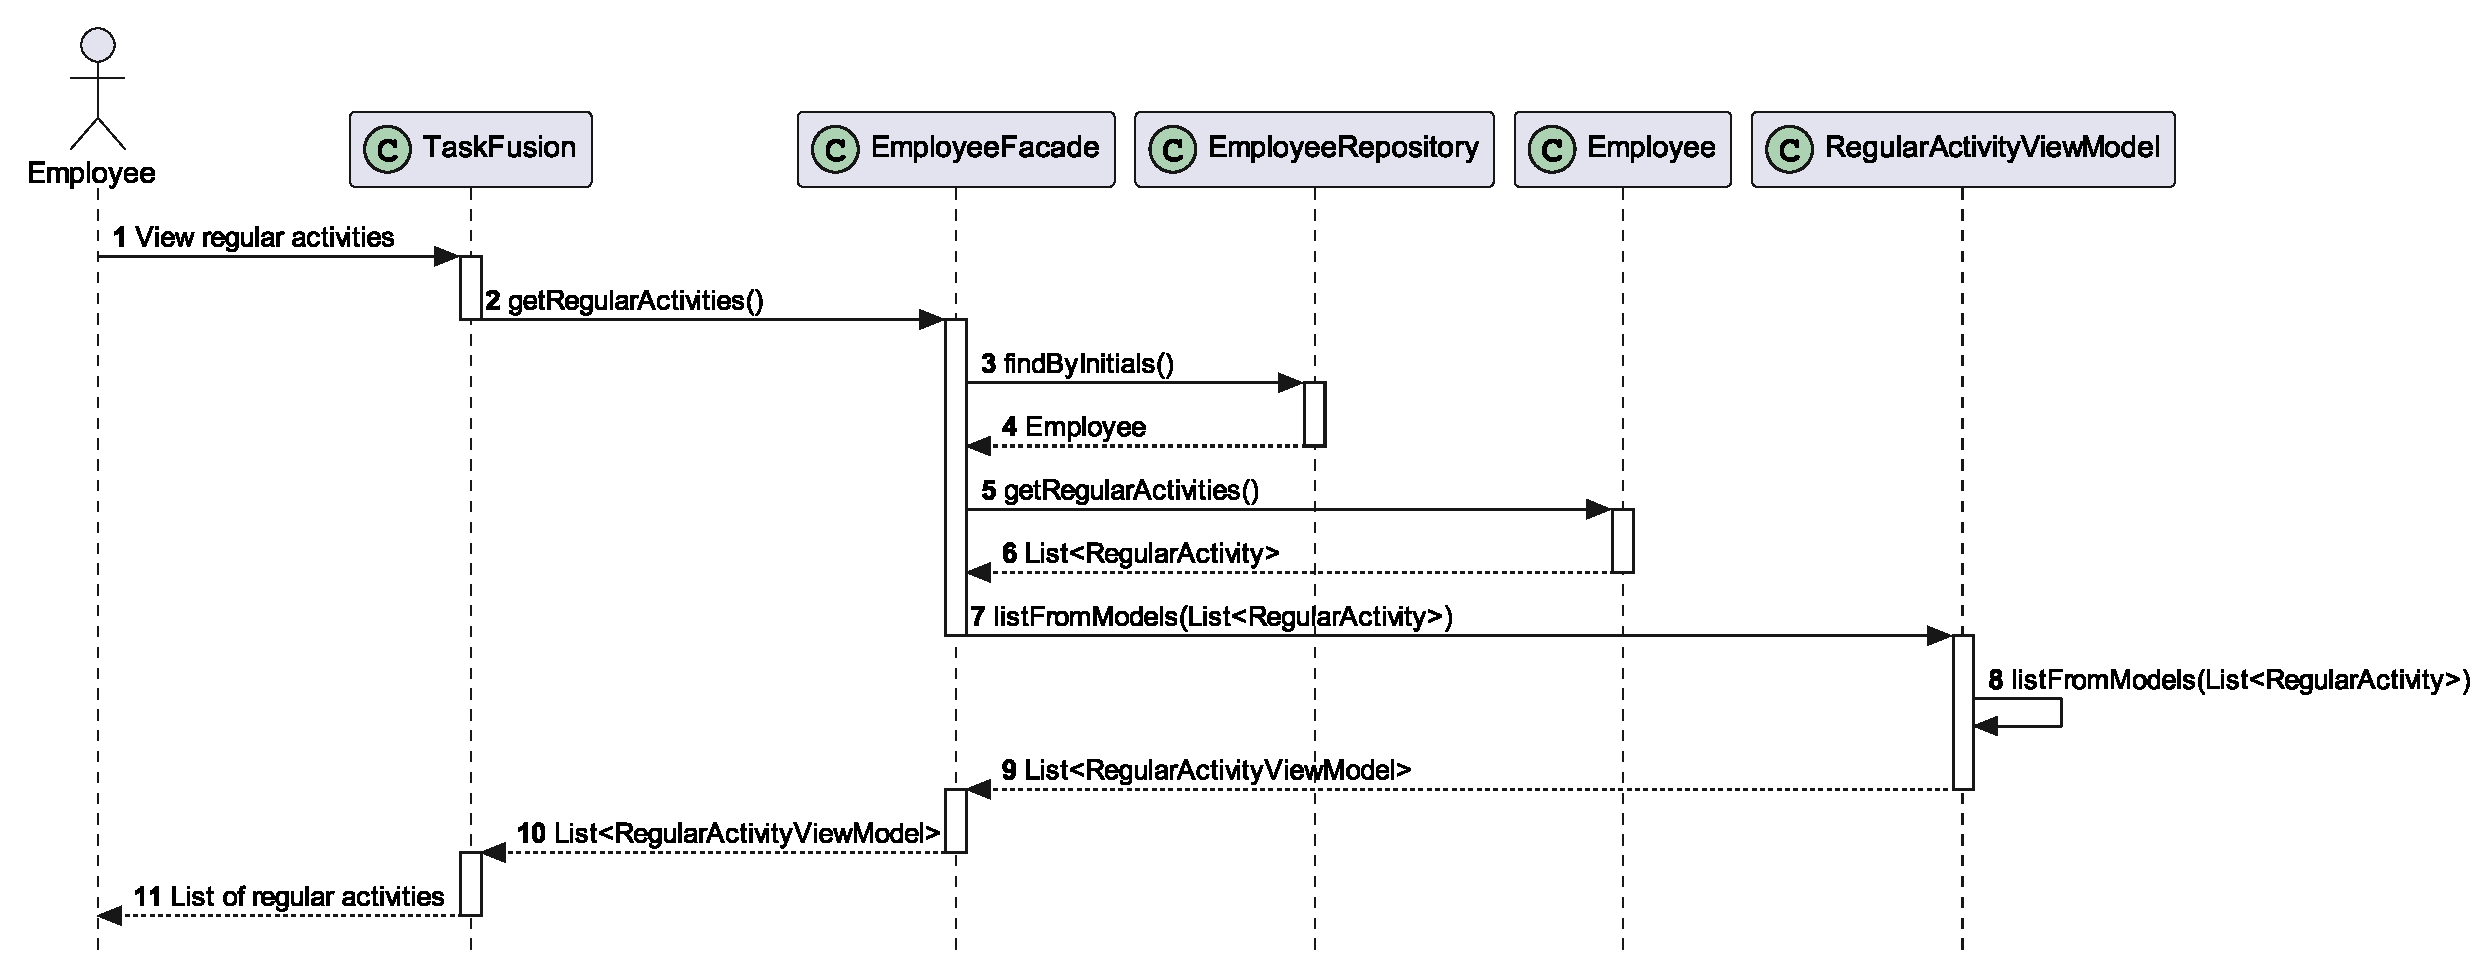
\includegraphics[width=\textwidth]{RequirementsAndDesign/SequenceDiagrams/seqViewRegularActivity.eps}
\end{figure}
\begin{figure}[H]
    \centering
    \caption{Sekvensdiagram: Registrer arbejdstid}\label{fig:sequenceRegisterWorktime}
    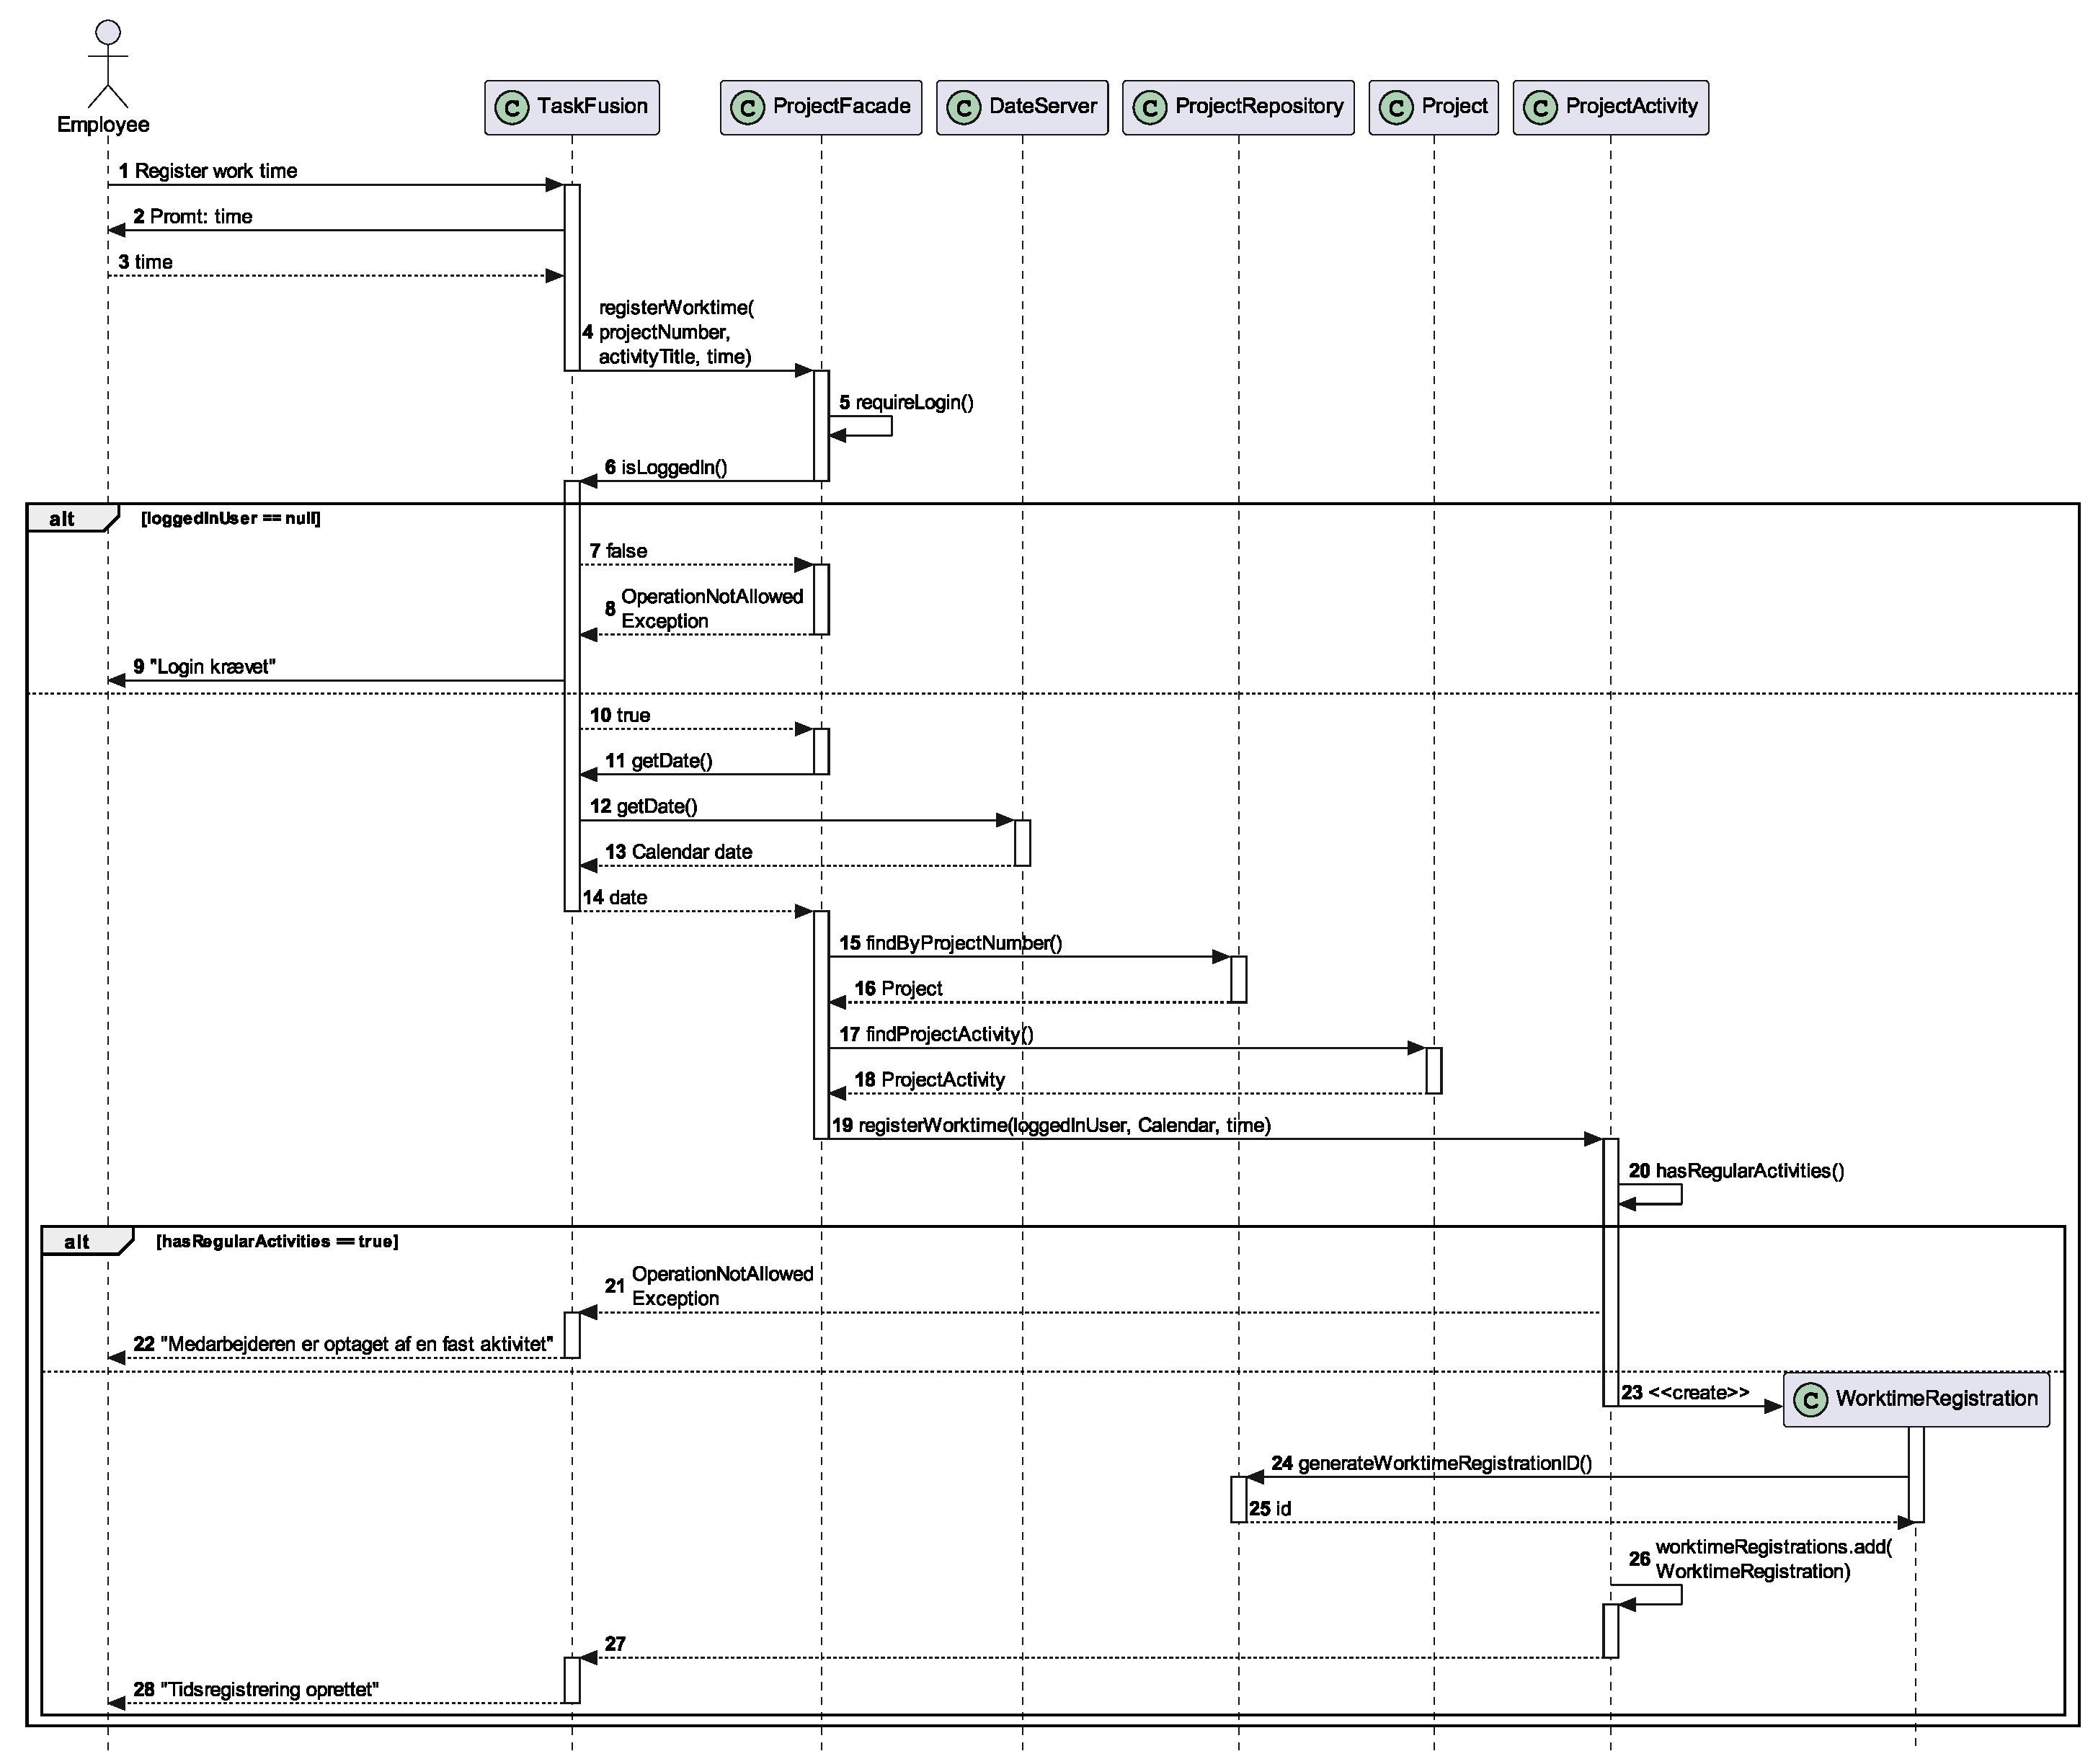
\includegraphics[width=\textwidth]{RequirementsAndDesign/SequenceDiagrams/seqRegisterWorktime.eps}
\end{figure}
\begin{figure}[H]
    \centering
    \caption{Sekvensdiagram: Se registreret arbejdstid på projektaktivitet}\label{fig:sequenceViewWorktime}
    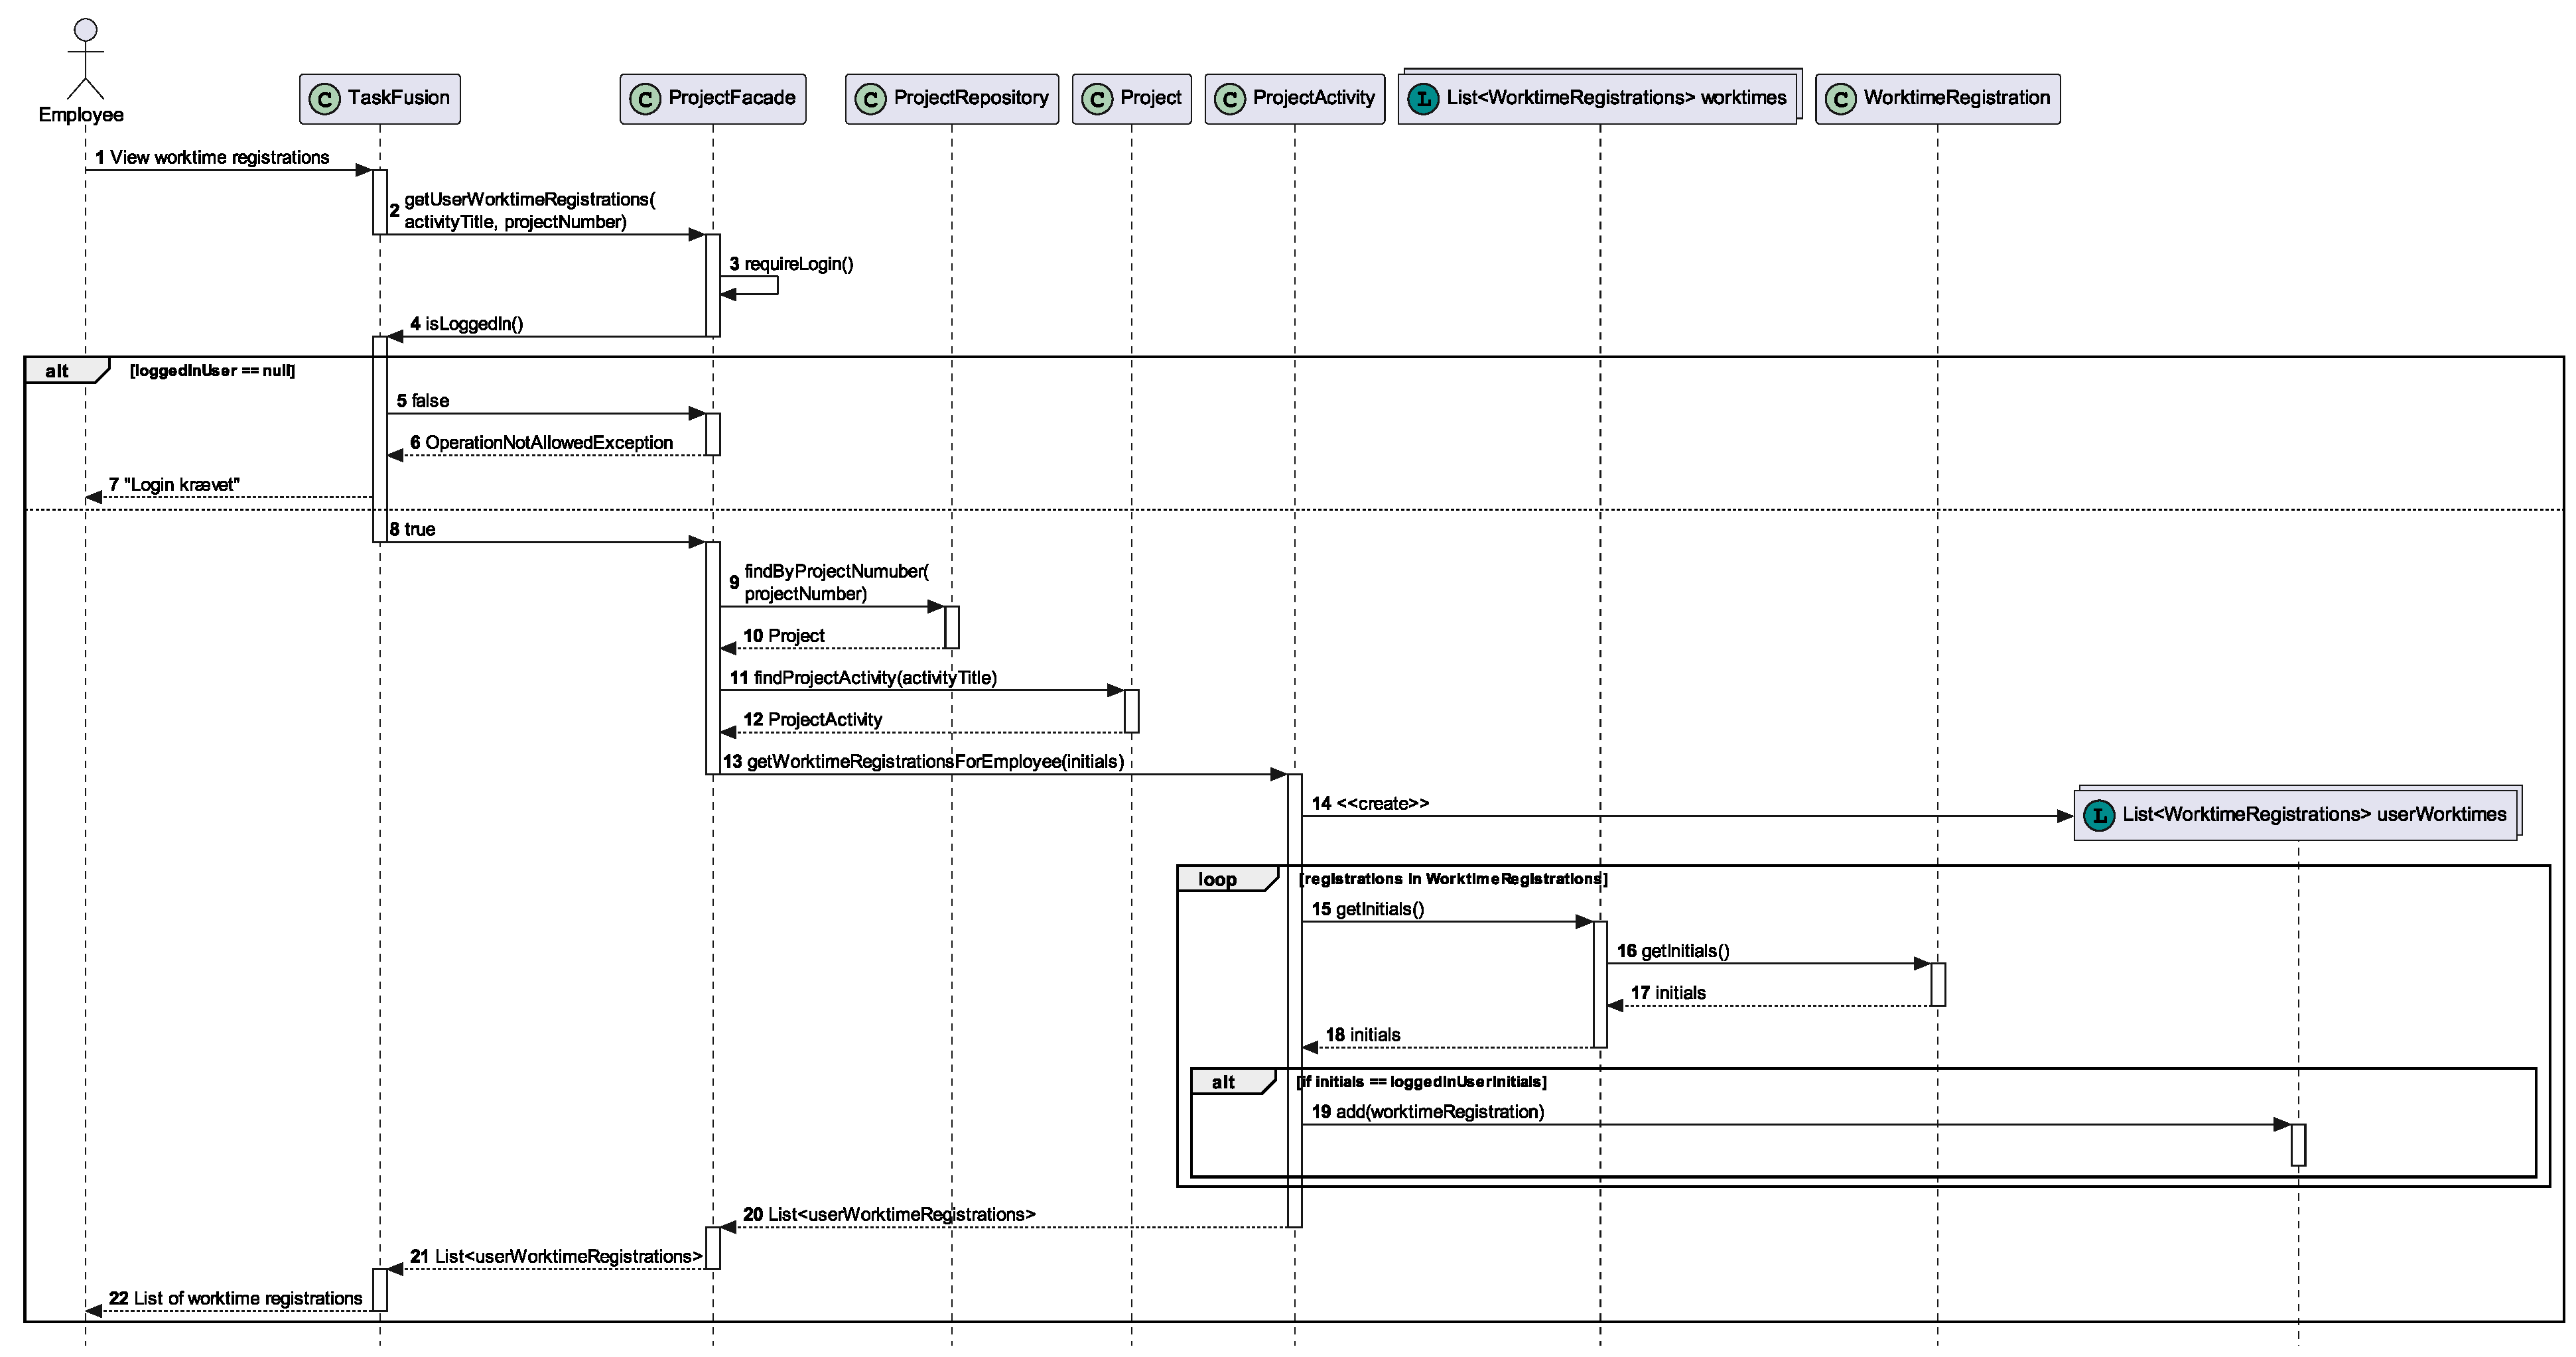
\includegraphics[width=\textwidth]{RequirementsAndDesign/SequenceDiagrams/seqViewWorktime.eps}
\end{figure}
\begin{figure}[H]
    \centering
    \caption{Sekvensdiagram: Generér projektrapport}\label{fig:sequenceGenerateProjectReport}
    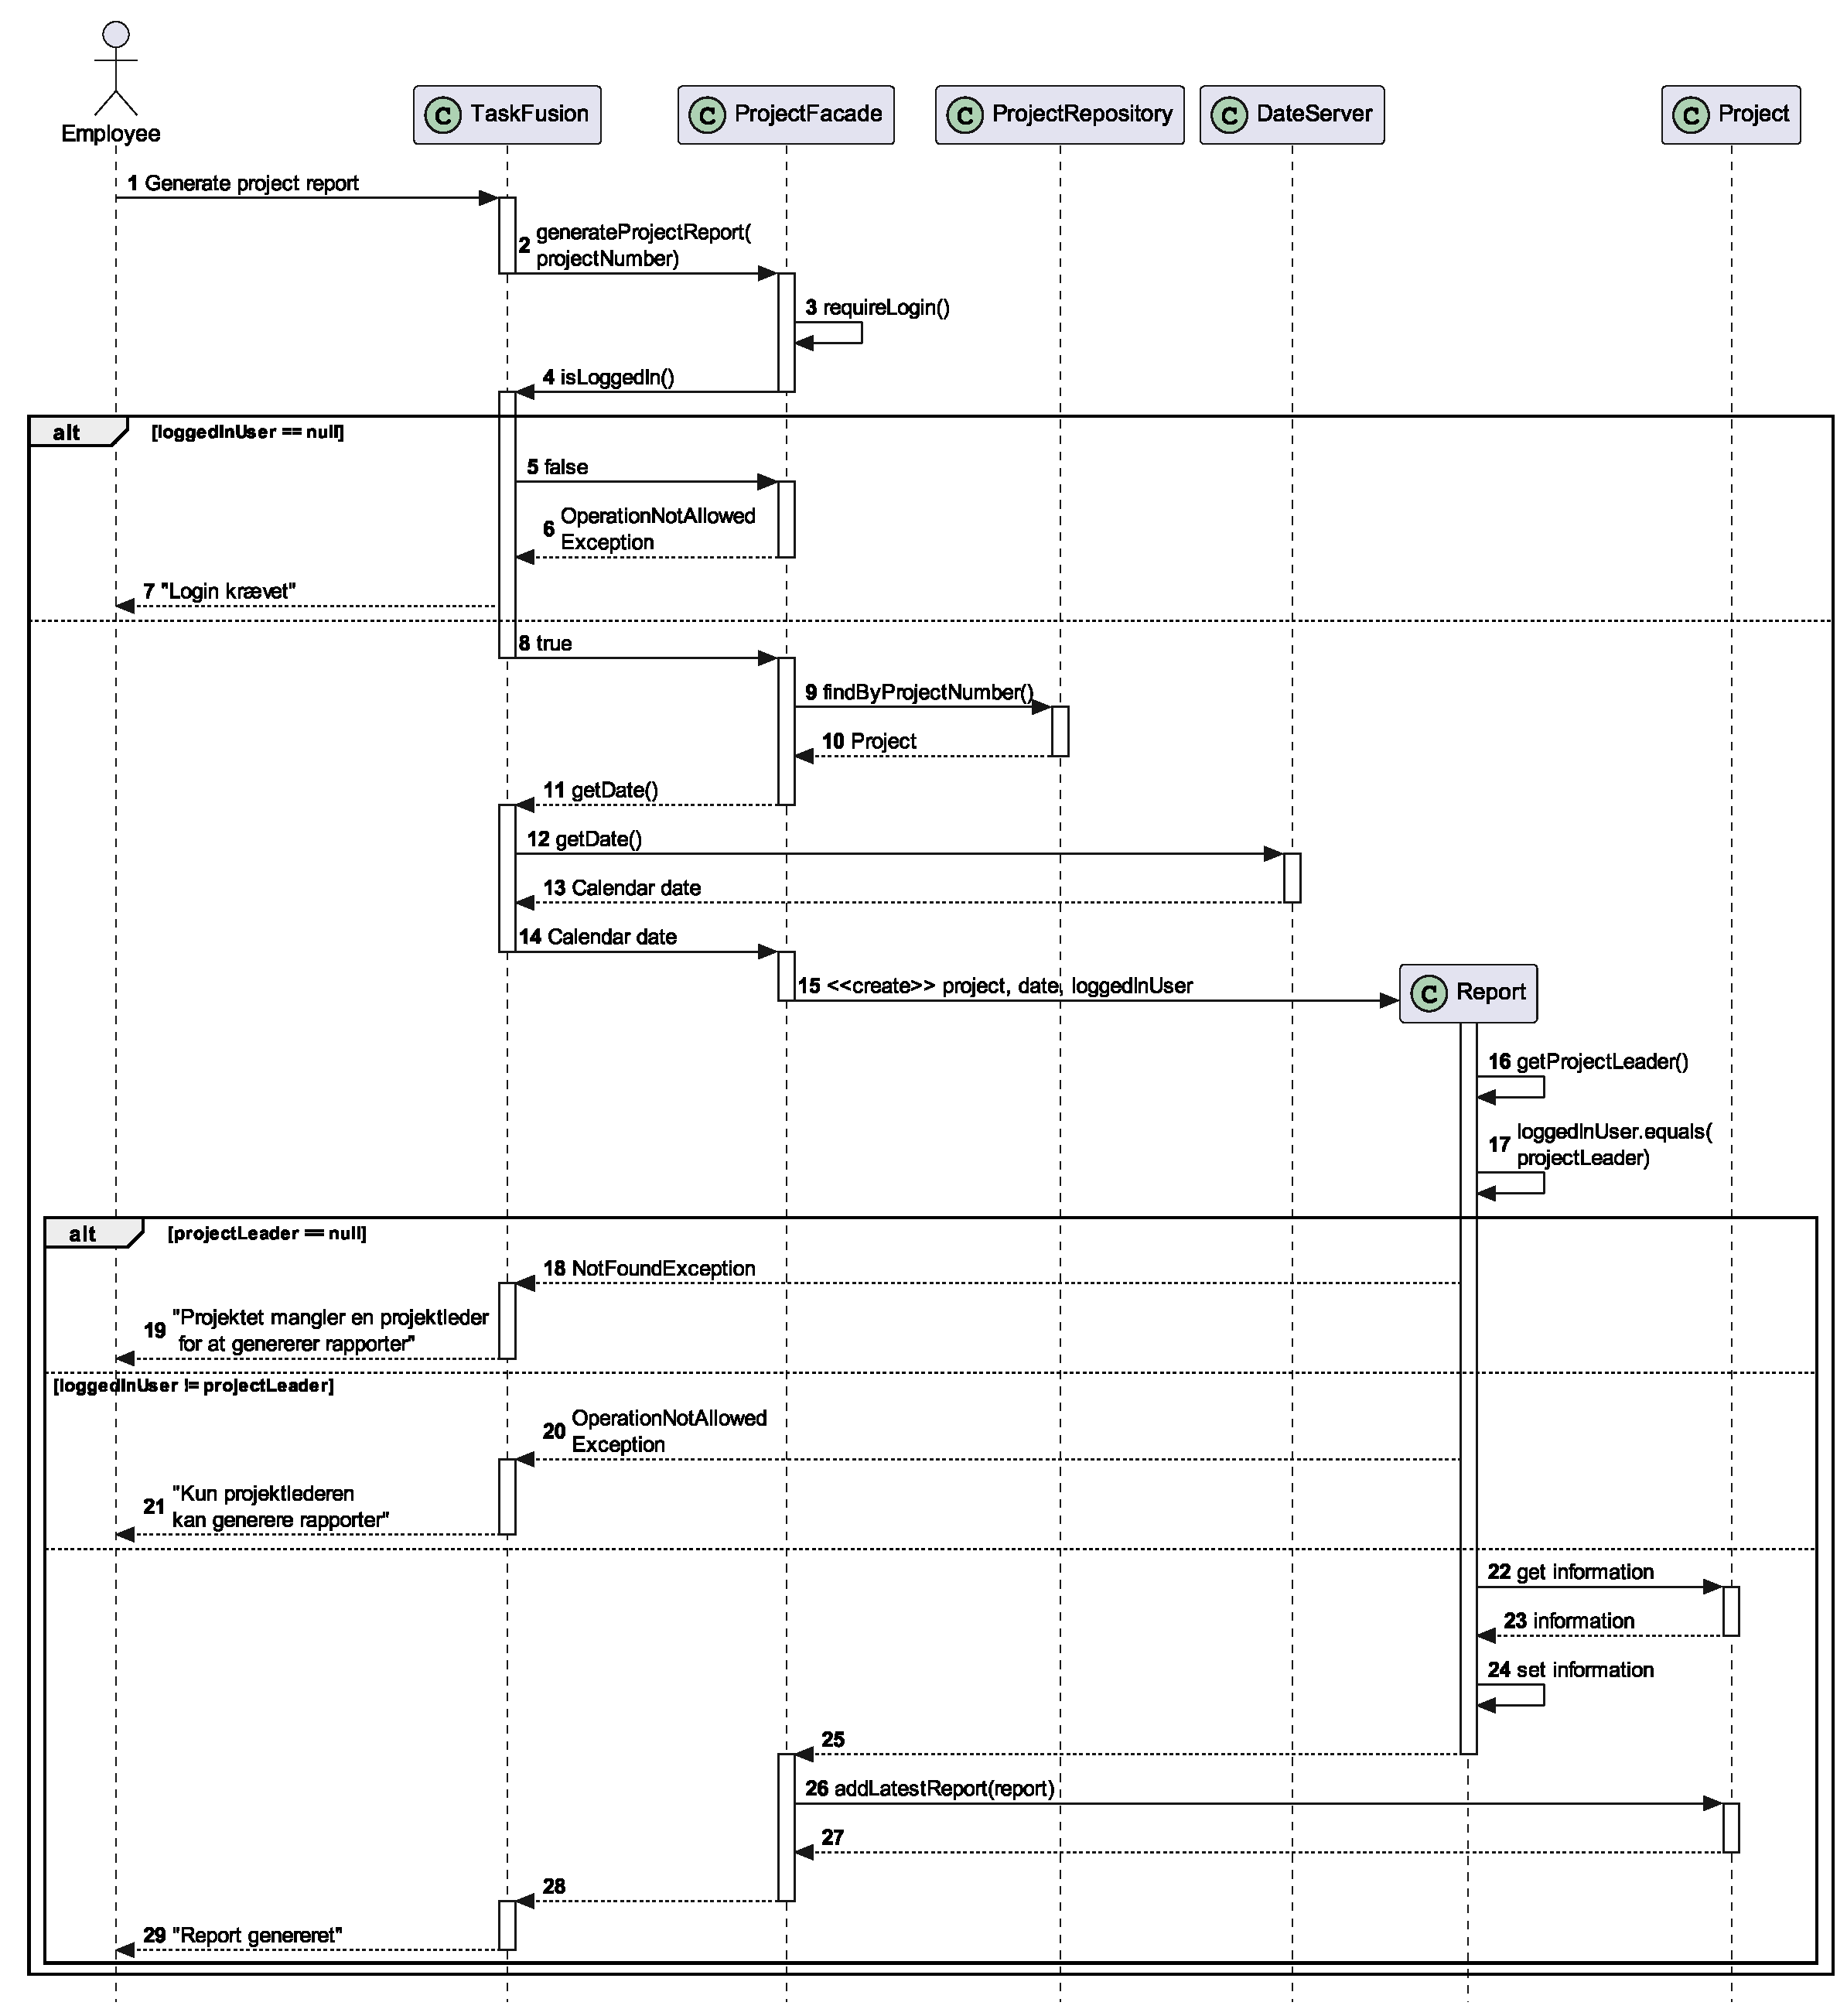
\includegraphics[width=\textwidth]{RequirementsAndDesign/SequenceDiagrams/seqGenerateProjectReport.eps}
\end{figure}
\section{Diskussion: Programdesign}
I dette afsnit bearbejdes to ting kort:
\begin{enumerate}
    \item Valg af datastrukturer
    \item Valg af klassestrukturer
\end{enumerate}
\subsection{Datastrukturer} I valg af datastrukturer er det vigtigt hvorledes vi henter og gemmer data. I programmet bliver medarbejdere og aktiviteter defineret med en unik streng, mens projekter bliver defineret med et løbenummer. Hvis man for nemheds skyld konverterer løbenummeret til en streng, er der mulighed for, at alle tre objekter kan gemmes i Map strukturer. Dette gør det nemt at hente objekter med \mintinline{java}|.get(key)|, udføre operationer på objekterne og overskrive objekterne i Map'et med \mintinline{java}|.put(key, Object)|. Er det nødvendigt at iterere over et Map, kan man også nemt bruge Java's \mintinline{java}|.stream()| metode. Ønsker man at gemme brugt arbejdstid på en aktivitet, er det derimod nemmest at gemme denne i en List, da arbejdstiden kun akkumuleres.
\subsection{Klassestrukturer} 
Programmet skal holdes simpelt og objekter skal nødvendigvis eje hinanden på en simpel måde. Desuden vil der være fokus på at adskille præsentationslag, businesslag og persistency så meget som muligt, således at lav kobling såvel som en overskuelig programstruktur opnås. Selve UI'en vil være en CLI (\textit{command-line-interface}) hvor en struktur bestående af \textit{view}-klasser haves. Yderligere benyttes \textit{facades} til at samle business-lagets funktioner, hvilket gør det let at hente processeret data. Persistency er delt op i to større kategorier: Employees (\textit{EmployeeRepository.java}) og alt vedr. projekter og deres aktiviteter (\textit{ProjectRepository.java}).